%%%%%%%%%%%%%%%%%%%%%%%%%%%%%%%%%%%%%%%%%%%%%%%%%%%%%%%%%%%%%%%%%%%%%%%%%%%%%%%%%%%%%%
%%%%%%%%%%%%%%%%%%%%%%%%%%%%%%%%%%%%%%%%%%%%%%%%%%%%%%%%%%%%%%%%%%%%%%%%%%%%%%%%%%%%%%
\section{\KL\ expansion}\label{fieldgeneratio}
%%%%%%%%%%%%%%%%%%%%%%%%%%%%%%%%%%%%%%%%%%%%%%%%%%%%%%%%%%%%%%%%%%%%%%%%%%%%%%%%%%%%%%
%%%%%%%%%%%%%%%%%%%%%%%%%%%%%%%%%%%%%%%%%%%%%%%%%%%%%%%%%%%%%%%%%%%%%%%%%%%%%%%%%%%%%%

Due to incomplete knowledge about the rock properties that show variability at multiple length scales, input parameters such as the permeability field, $\perm(\vx,\ale)$, are treated as random space functions with statistics inferred from geostatistical models (here $\vx =\left( x_{1},x_{2},x_{3}  \right)^{\! ^{\mathsf{T}}}\in \mathbb{R}^{3}$ and $\ale$ is a random element in the probability space).
In line with \cite{dagan89} and \cite{gelhar93} the permeability field is modeled as a log-normally distributed random space function
%
\begin{equation}
  \perm\fxw = \beta\exp\Big[\rho\Y\fxw\Big],
\label{field}
\end{equation}
%
\noindent where $\beta,\rho\in\mathbb{R}^{+}$ and $\Y\fxw \sim \normalf{\me{\Y}}{\covn{\Y}}$ is a Gaussian random field
characterized by its mean $\me{\Y} = \med{\Y}$ and two-point covariance function

\begin{equation}
 \covv{\Y} = \covar{\Y\fx}{\Y\fy} = \mathsf{E}\Big[ \big( \Y\fx - \med{\Y\fx}  \big) \big( \Y\fy - \med{\Y\fy}  \big) \Big].
 \label{covg}
\end{equation}
%
\textcolor{black}{Moreover, in this work, $\Y$ is a second-order stationary process\index{second-order stationary process} \citep{gelhar93}, that is:}

\begin{equation}
 \begin{array}{rcl}
    \med{\Y\fx} &=& \me{\Y},\quad \mbox{(constant)}\\ \\
    \covv{\Y}   &=& \covn{\Y}\left(\lVert \vx - \vy \rVert \right) = \covn{\Y}\left(d\right).
 \end{array}
\end{equation}


The Gaussian field $\Y$ can be represented as a series expansion involving a complete set of deterministic functions with correspondent random coefficients using the \KL\ (\kl) expansion proposed independently by \cite{karhunen46} and \cite{loeve55}.
It is based on the eigen-decomposition of the covariance function.
Depending on how fast the eigenvalues decay one may be able to  retain only a small number of terms in a truncated expansion and, consequently, this procedure may reduce the search to a smaller parameter space.
In uncertainty quantification methods for porous media flows, the \kl\ expansion has been widely used to reduce the number of parameters used to represent the permeability field \citep{efendiev05,efendiev2006,das10,mondal10,ginting11,ginting12}.
Another advantage of \kl\ expansion lies on the fact that it provides orthogonal deterministic basis functions and uncorrelated random coefficients, allowing for the optimal encapsulation of the information contained in the random process into a set of discrete uncorrelated random variables \citep{GhanemSpanos}.
This remarkable feature can be used to simplify the Metropolis-Hastings \mcmc\ Algorithm in the sense of the search may be performed in the space of discrete uncorrelated random variables ($\vtheta$), no longer in the space of permeabilities which have a more complex statistical structure.

%%%%%%%%%%%%%%%%%%%%%%%%%%%%%%%%%%%%%%%%%%%%%%%%%%%%%%%%%%%%%%%%%%%%%%%%%%%%%%%%%%%%%%%%%%%%%%%%%%%%%%%%%%%%%%%%%%%%%%%%%%%%%%%%%%%%
%%%%%%%%%%%%%%%%%%%%%%%%%%%%%%%%%%%%%%%%%%%%%%%%%%%%%%%%%%%%%%%%%%
Here we recall the basic facts about the \KL\ expansion.
Consider a random field $\Y(\vx,\ale)$ defined on a probability space $(\Omega,\events,\probab)$ composed by the sample space, the ensemble of events and a probability measure, respectively, and indexed on a bounded domain $\D \in \mathbb{R}^{3}$.
The process $\Y$ can be expressed as
%
\begin{equation}
  \Yxw = \med{\Y(\vx)} +\sum_{i=1}^{\infty}\sqrt{\avai} \avei(\vx)
\theta_{i}(\ale),
\label{kl}
\end{equation}
%
\noindent where $\avai$ and $\avei$ are the eigenvalues and eigenfunctions of the covariance function $\covv{\Y}$, respectively.
By definition, $\covv{\Y}$ is bounded, symmetric and positive definite and has the following eigen-decomposition:
%
\begin{equation*}
  \covv{\Y} = \sum_{i=1}^{\infty} \avai\avei(\vx)\avei(\vy).
\label{klcov}
\end{equation*}
%

The eigenvalues and eigenfunctions of \eq{kl} are the solution of the homogeneous Fredholm integral equation of second kind given by
%
\begin{equation}
  \int_{\D} \covv{\Y} \ave(\vx) d\vx = \ava\ave(\vy).
\label{fred}
\end{equation}
%
\noindent The solution of \eq{fred} forms a complete set of a square-integrable
orthogonal eigenfunctions that satisfy the equation
%
\begin{equation*}
  \int_{\D} \avei(\vx) \avej(\vx)=\delta_{ij},
\label{ortho}
\end{equation*}
%
\noindent in which $\delta_{ij}$ is the Kronecker-delta function.
$\theta_{i}(\ale)$ is a set of independent random variables which
can be expressed as
%
\begin{equation*}
  \theta_{i}(\ale) = \displaystyle
\frac{1}{\sqrt{\avai}}\int_{\D}\flu{\Y}\avei(\vx) d\vx,
\end{equation*}
%
\noindent where $\flu{\Y}=\Y-\med{\Y}$ is the fluctuation.
For practical implementations of the \kl\ expansion the eigenvalues are arranged from the largest to smallest and the series is approximated by a finite number of terms, say the first $\mm$, giving
%
\begin{equation}
  \Y\fxw \approx \med{\Y(\vx)} +\sum_{i=1}^{\mm}\sqrt{\avai} \avei(\vx)
\theta_{i}(\ale).
\label{klM}
\end{equation}
%
The corresponding covariance function is given by
%
\begin{equation*}
  \covv{\Ym} = \sum_{i=1}^{\mm} \avai\avei(\vx)\avei(\vy).
\label{klcovM}
\end{equation*}
%

The factors affecting the convergence of the \KL\ series are the ratio of the length of the process over correlation parameter, the form of the covariance function, and the solution method for the eigensolutions of the covariance function (see \cite{huang01}).
Next we discuss the field conditioning using the \kl\ expansion.

%%%%%%%%%%%%%%%%%%%%%%%%%%%%%%%%%%%%%%%%%%%%%%%%%%%%%%%%%%%%%%%%%%%%%%%%%%%%%%%%%%%%%%%%%%%%%%%%%%%%
%%%%%%%%%%%%%%%%%%%%%%%%%%%%%%%%%%%%%%%%%%%%%%%%%%%%%%%%%%%%%%%%%%%%%%%%%%%%%%%%%%%%%%%%%%%%%%%%%%%%
%%%%%%%%%%%%%%%%%%%%%%%%%%%%%%%%%%%%%%%%%%%%%%%%%%%%%%%%%%%%%%%%%%%%%%%%%%%%%%%%%%%%%%%%%%%%%%%%%%%%
The number of terms used in the series can be chosen based on the energy represented by the sum of the eigenvalues.
Then we define the relative energy for $n$ terms as

\begin{equation}
 \re{n} = \dfrac{\sum_{i=1}^{n}\avai}{\sum_{j=1}^{m\rightarrow\infty}\avaj}.
\end{equation}
%%%%%%%%%%%%%%%%%%%%%%%%%%%%%%%%%%%%%%%%%%%%%%%%%%%%%%%%%%%%%%%%%%%%%%%%%%%%%%%%%%%%%%
%%%%%%%%%%%%%%%%%%%%%%%%%%%%%%%%%%%%%%%%%%%%%%%%%%%%%%%%%%%%%%%%%%%%%%%%%%%%%%%%%%%%%%




The eigenvalues associated with the eigenfunctions provide
a measure of the energy contained in the respective mode.
%%%%%%%%%%%%%%%%%%%%%%%%%%%%%%%%%%%%%%%%%%%%%%%%%%%%%%%%%%%%%%%%%%%%%%%%%%%%%%%%%%%%%%
To quantify the energy involved in a truncated \kl\ expansion (with $\m$ modes) we define the total relative energy as
\begin{equation}
 \Enn{\m} = \dfrac{\sum_{j=1}^{\m}\avaj}{\sum_{i=1}^{m\rightarrow\infty}\avai},
\end{equation}

\noindent in which the denominator will be approximated by $m=30,000$ eigenvalues.


The \fig{eigenvalues} shows the behavior of the eigenvalues, the energy contained, and the average error as a function of the number of modes ($\m$) for the three covariance functions considered in this study.
The decay of the eigenvalues of the square exponential case is much faster than the exponential case. The latter requires a more significant number of modes to capture the same energy when compared to the first one.
%%%%%%%%%%%%%%%%%%%%%%%%%%%%%%%%%%%%%%%%%%%%%%%%%%%%%%%%%%%%%%%%%%%%%%%%%%%%%%%%%%%%%%
\begin{figure}[H]
 \centering
 \subfigure[Squared exponential covariance ($\clen= 0.1$)]{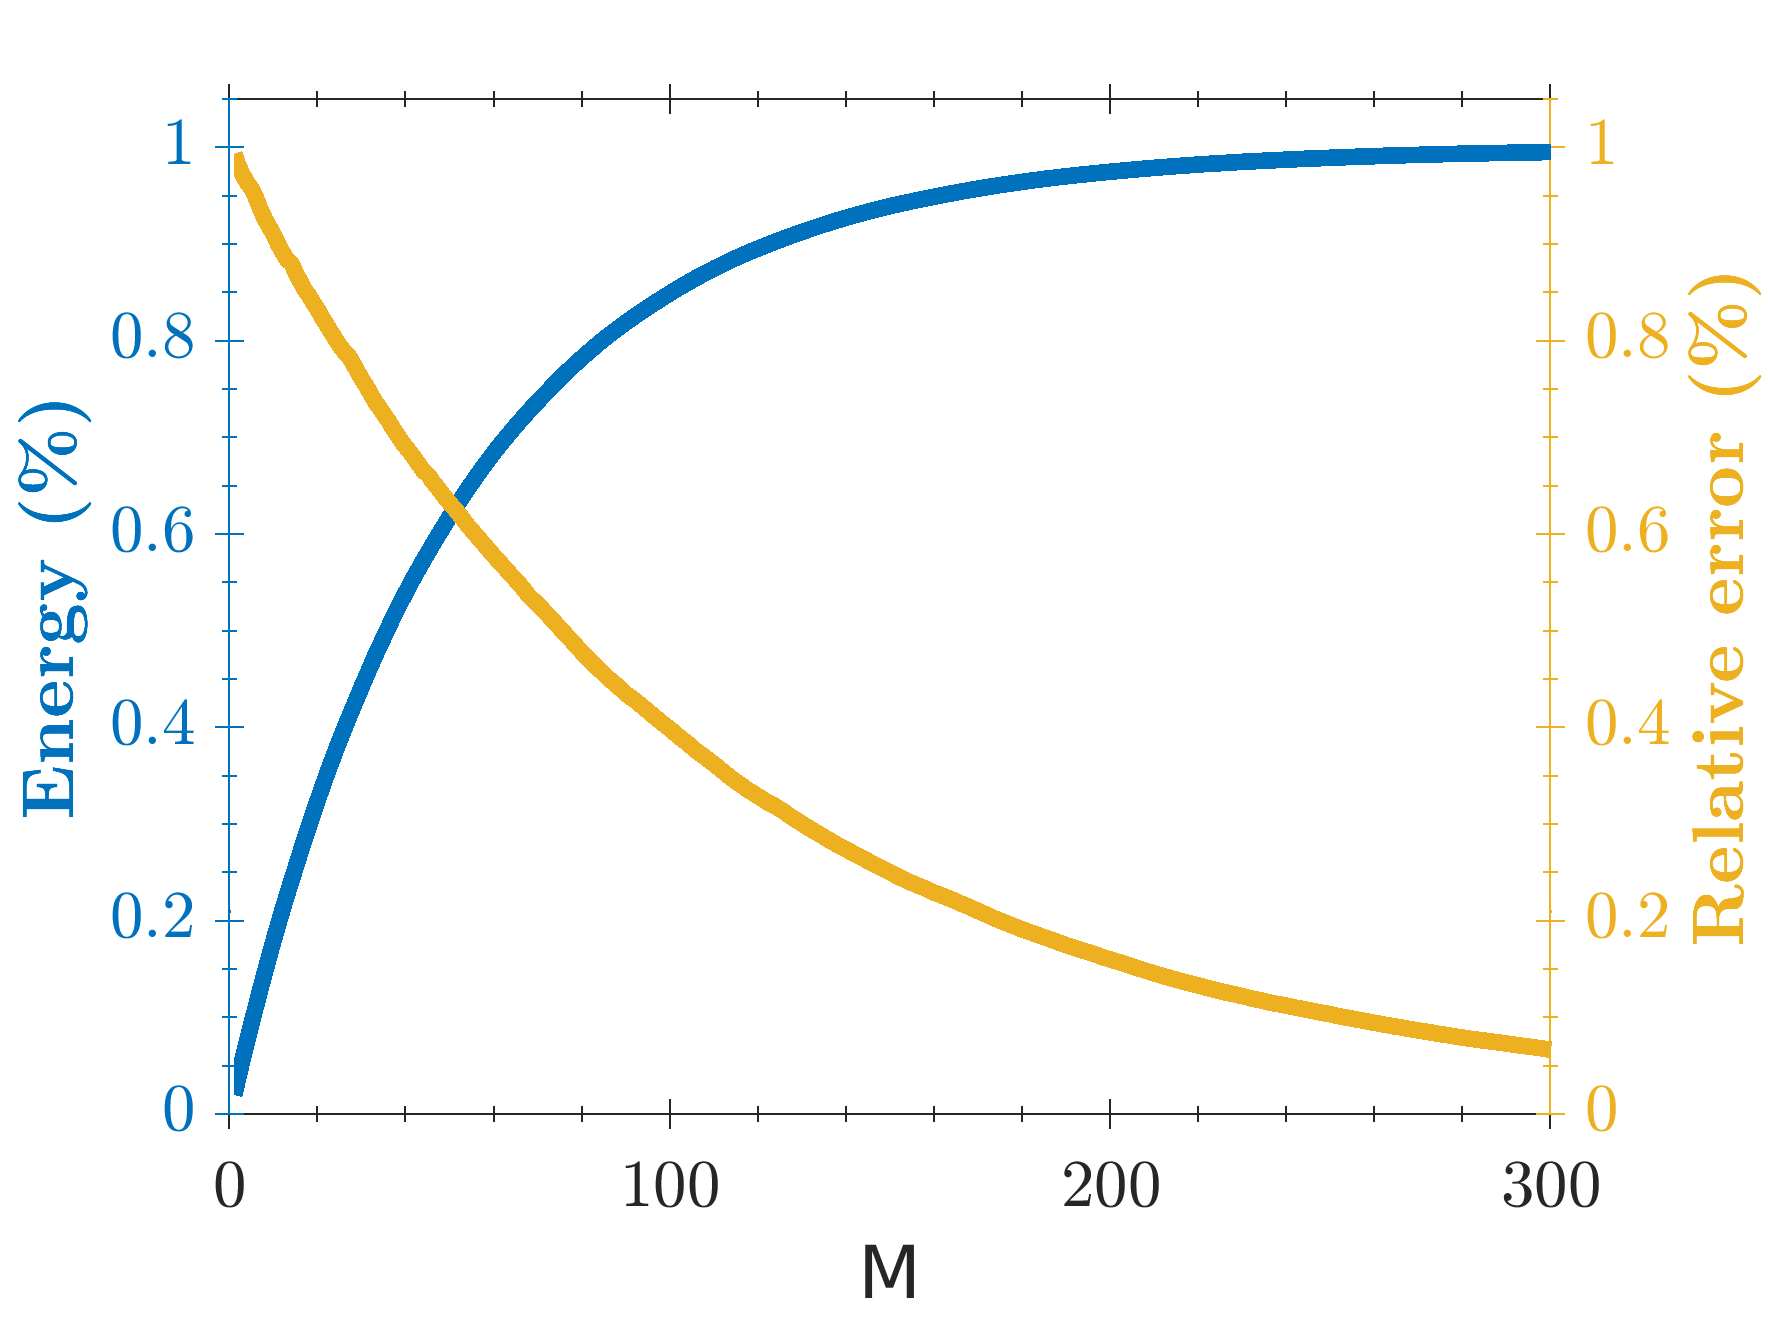
\includegraphics[scale=0.475]{./figuras/Energy_sexp_100x100x1_0-1x0-1_30000.png}
 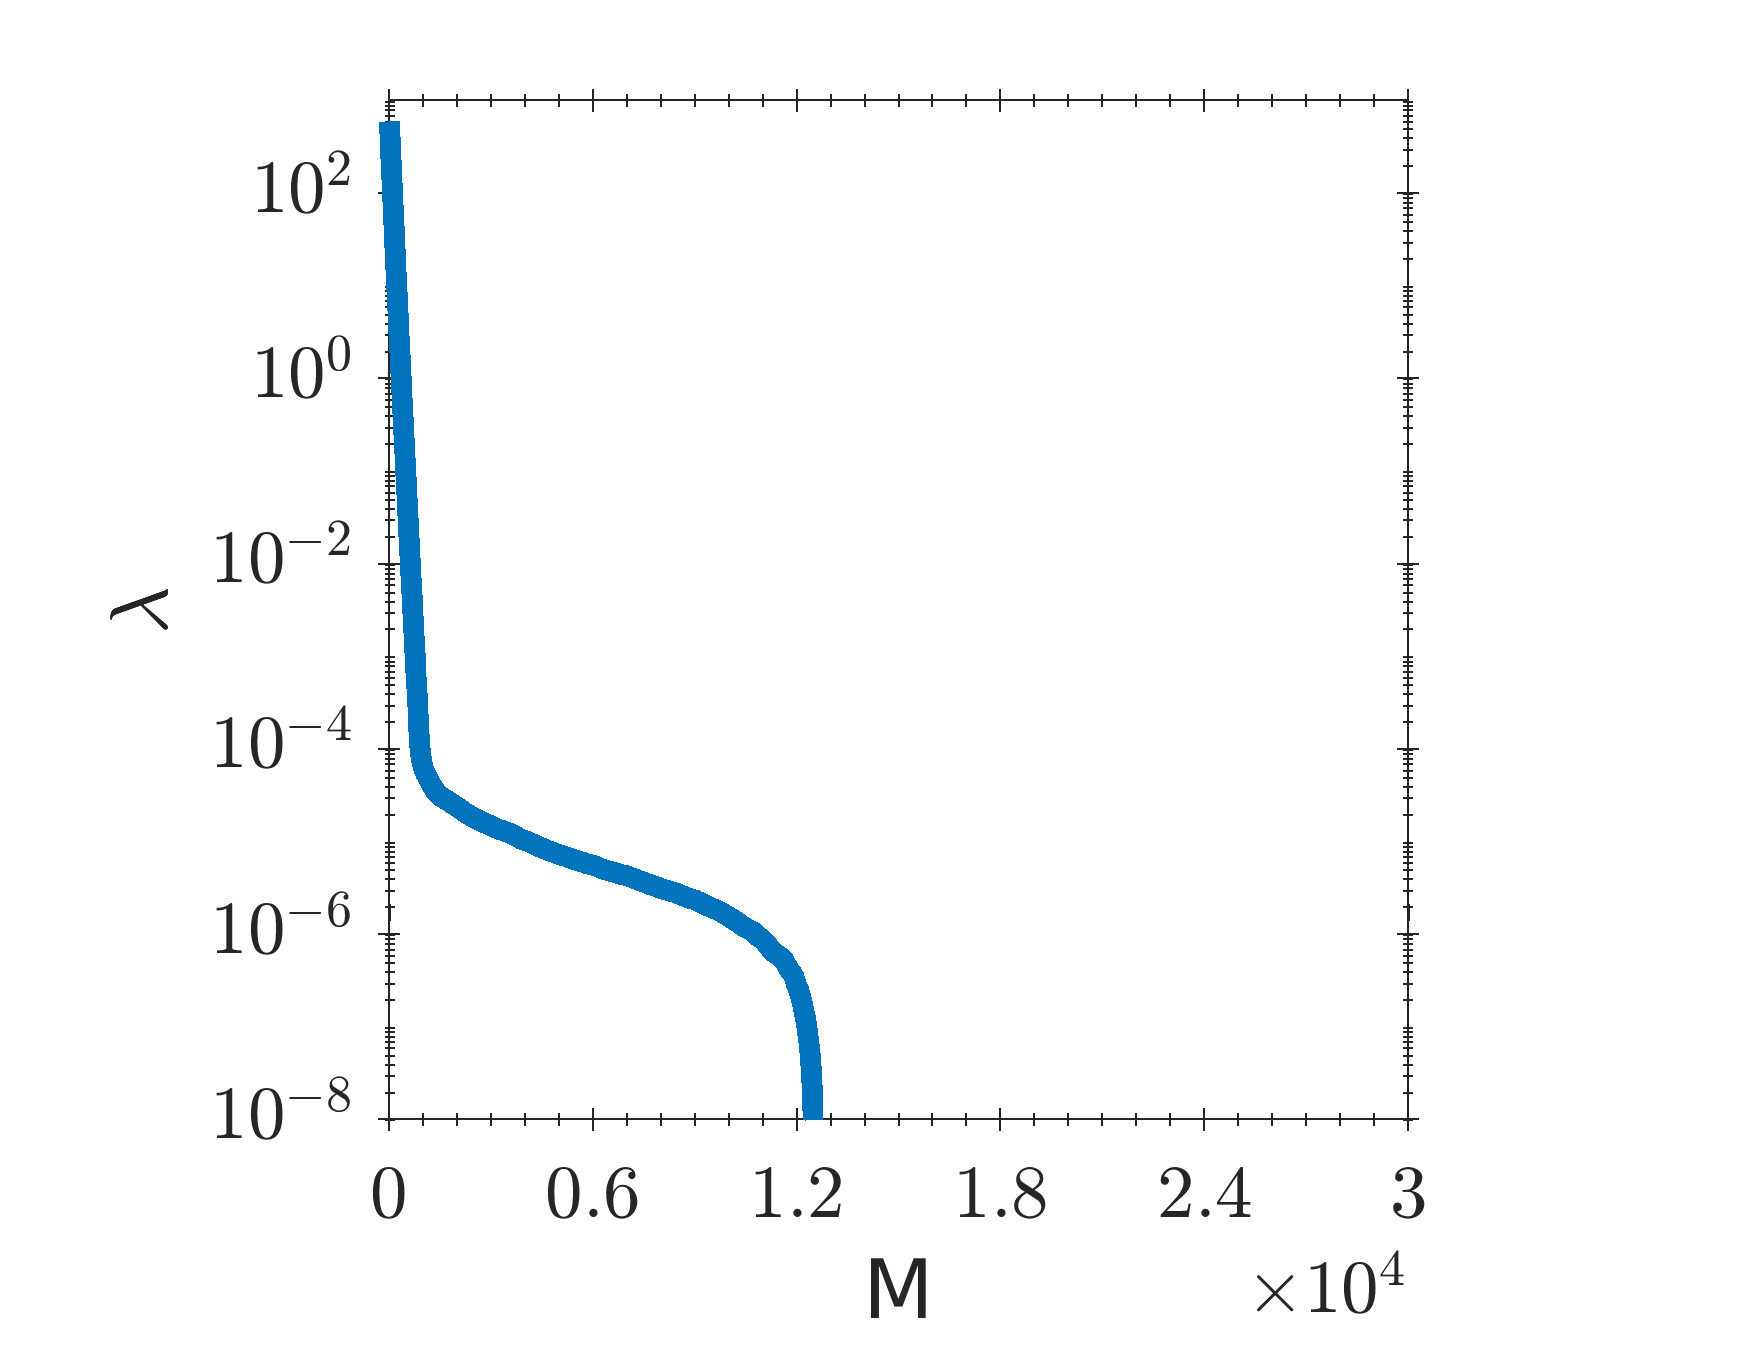
\includegraphics[scale=0.485]{./figuras/sexp_autoval_100x100x1_0-1x0-1_30000.png}}
 \subfigure[Exponential covariance ($\clen= 0.1$)]{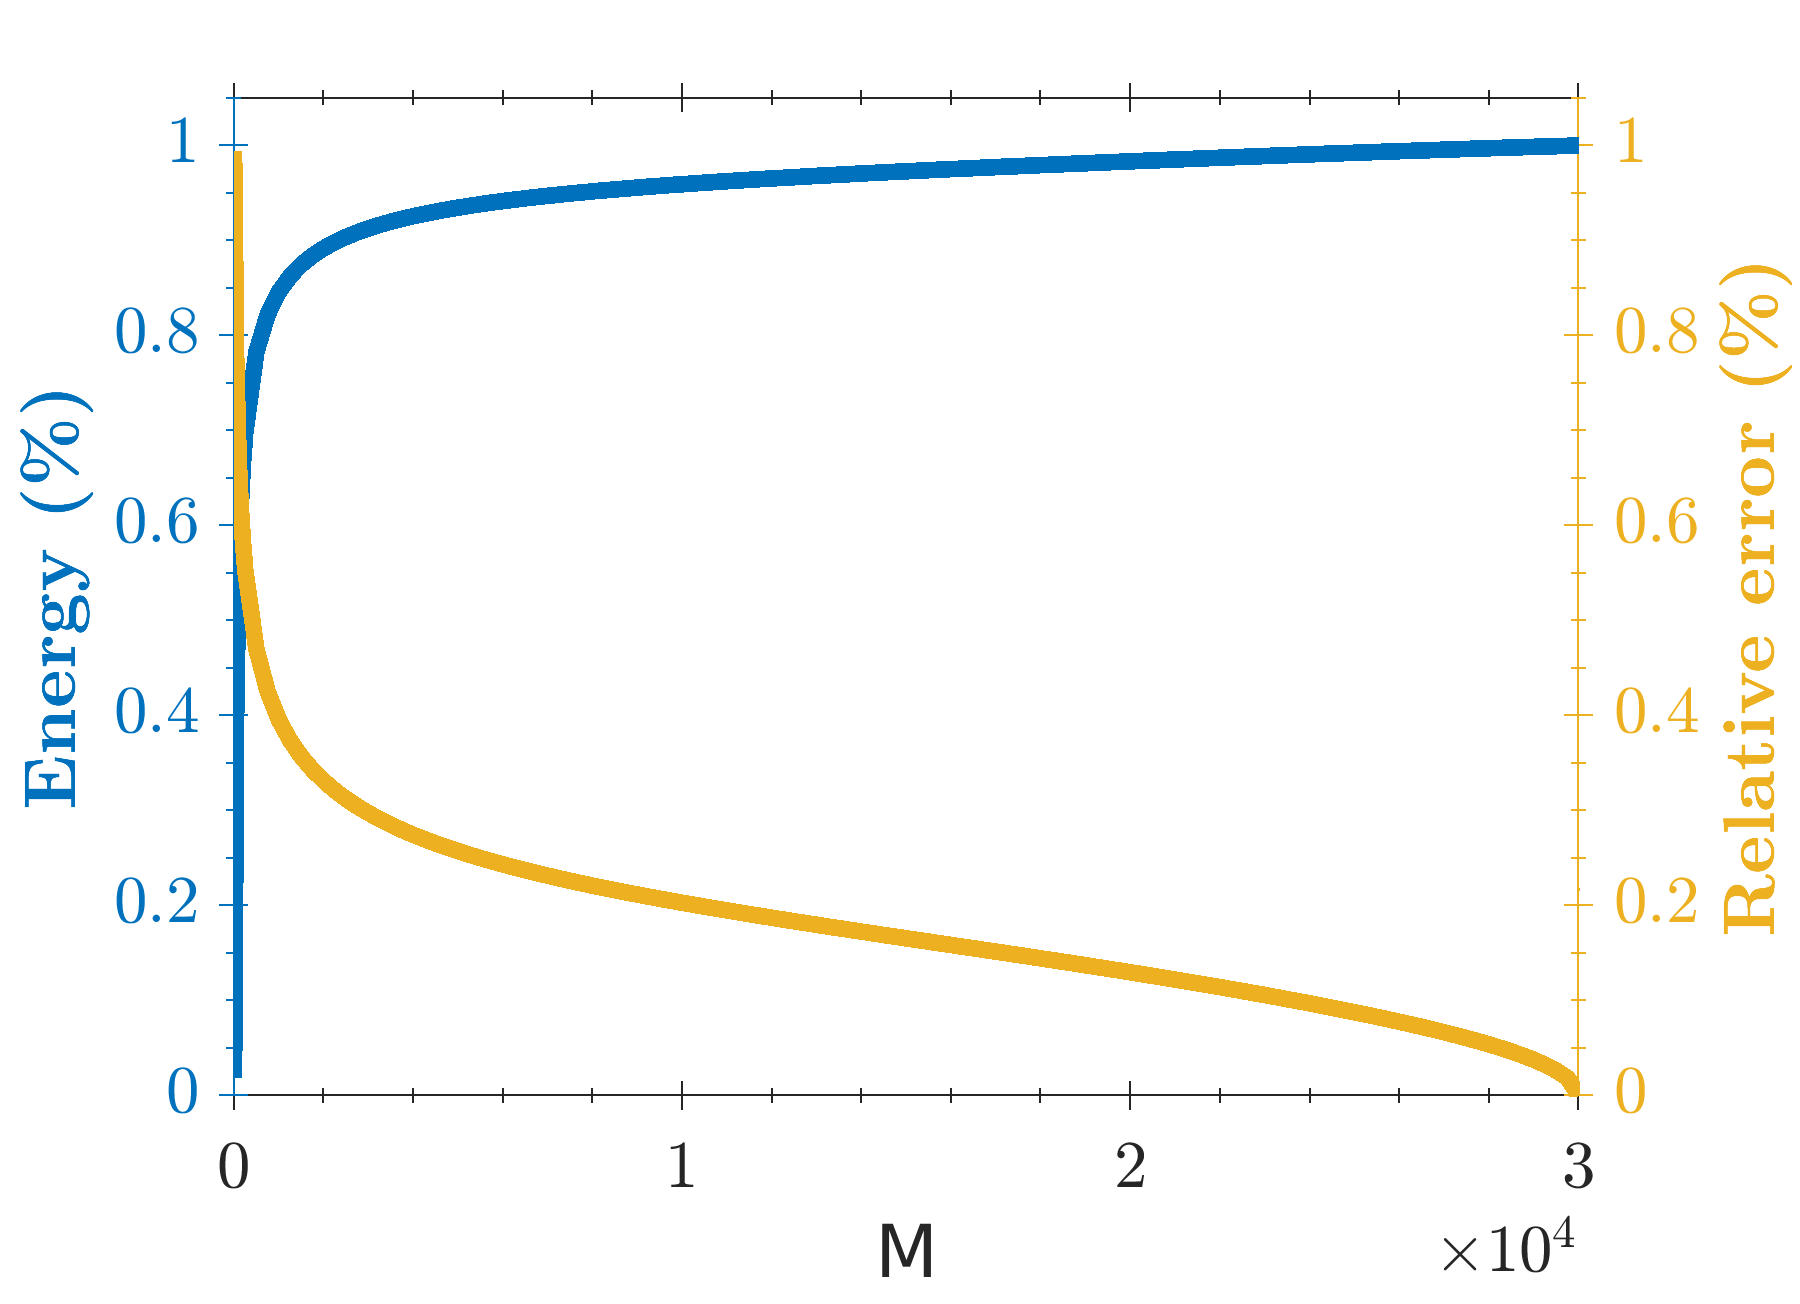
\includegraphics[scale=0.475]{./figuras/Energy_exp_100x100x1_0-1x0-1_30000.png}
 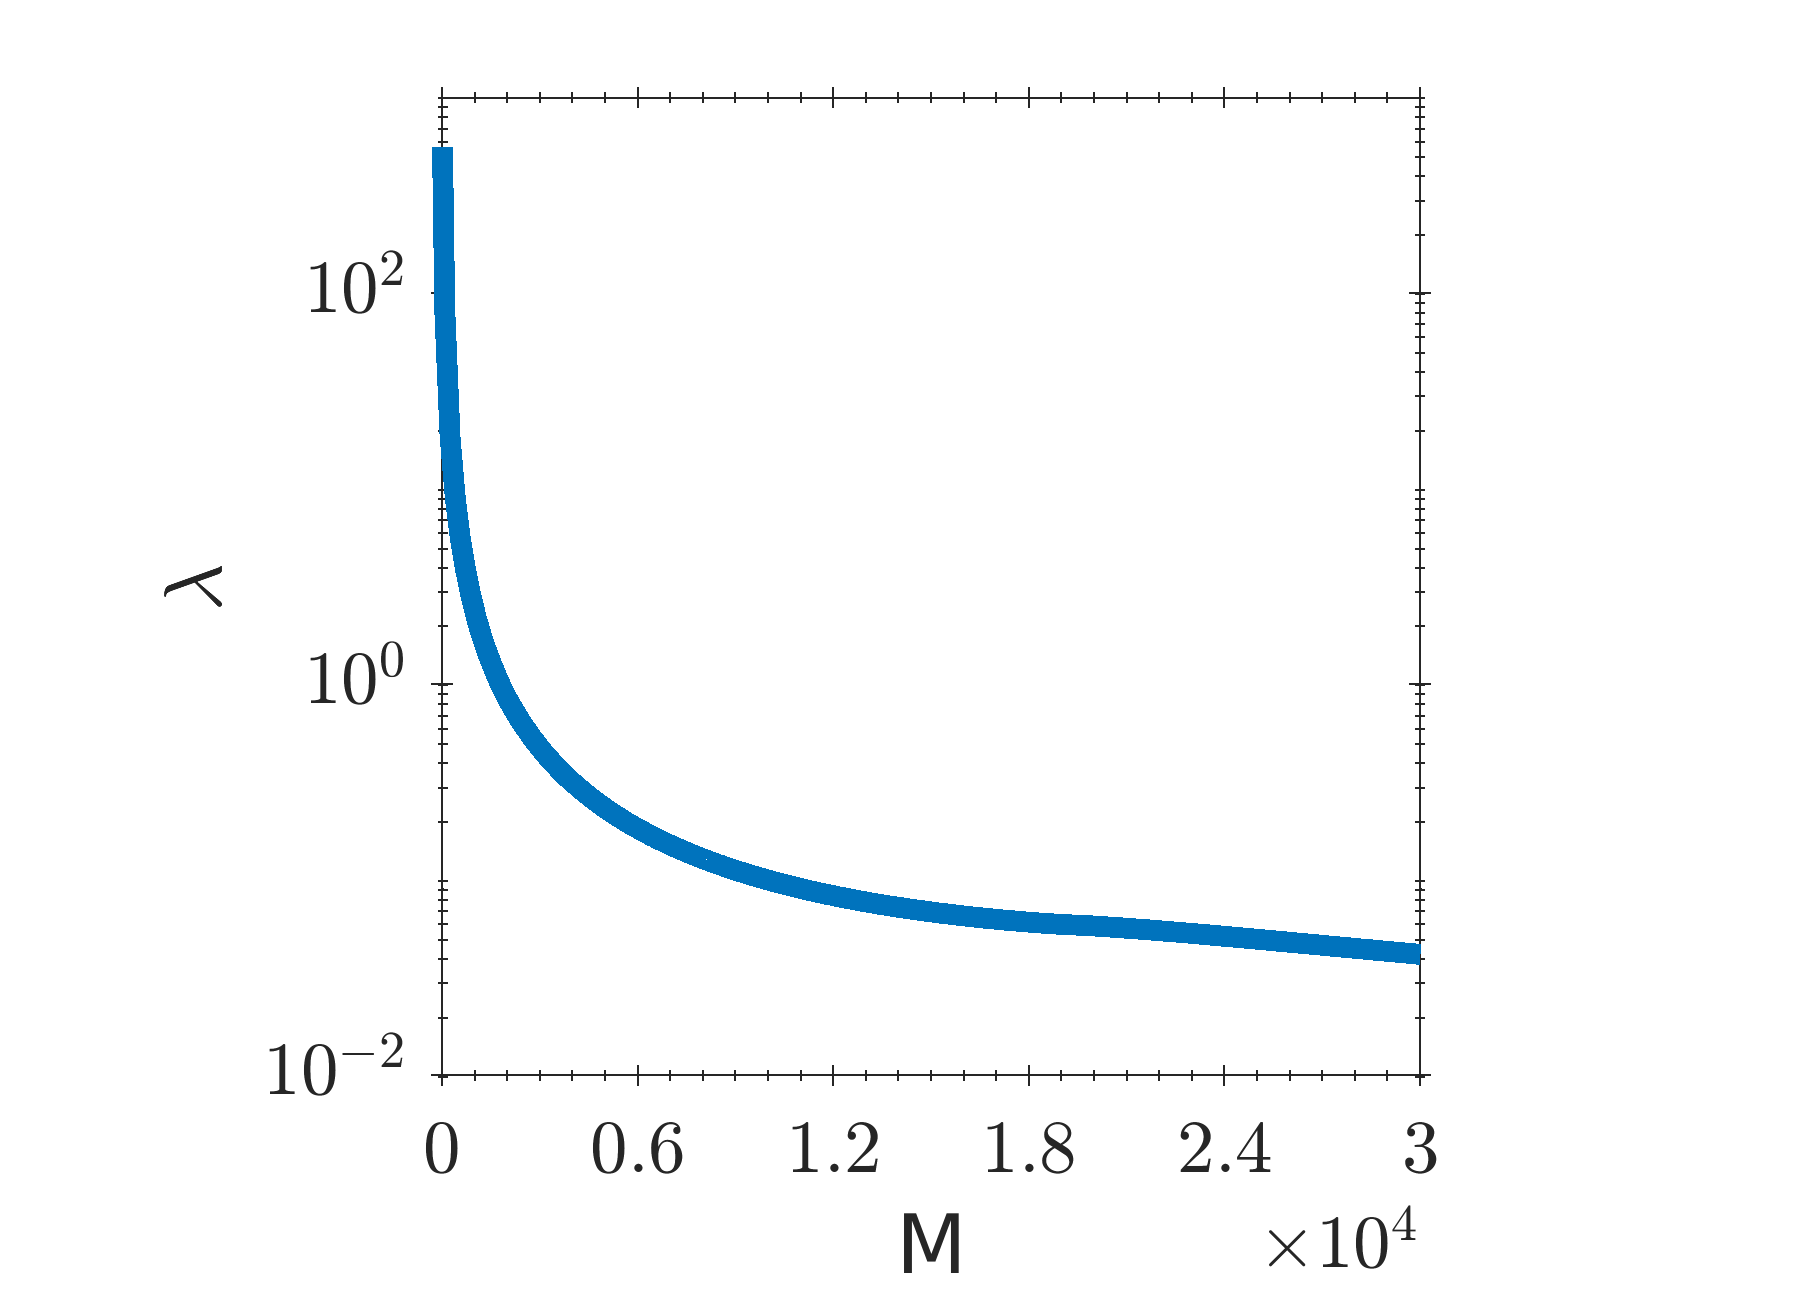
\includegraphics[scale=0.485]{./figuras/exp_autoval_100x100x1_0-1x0-1_30000.png}}\\
 \subfigure[Exponential covariance ($\clen= 0.2$)]{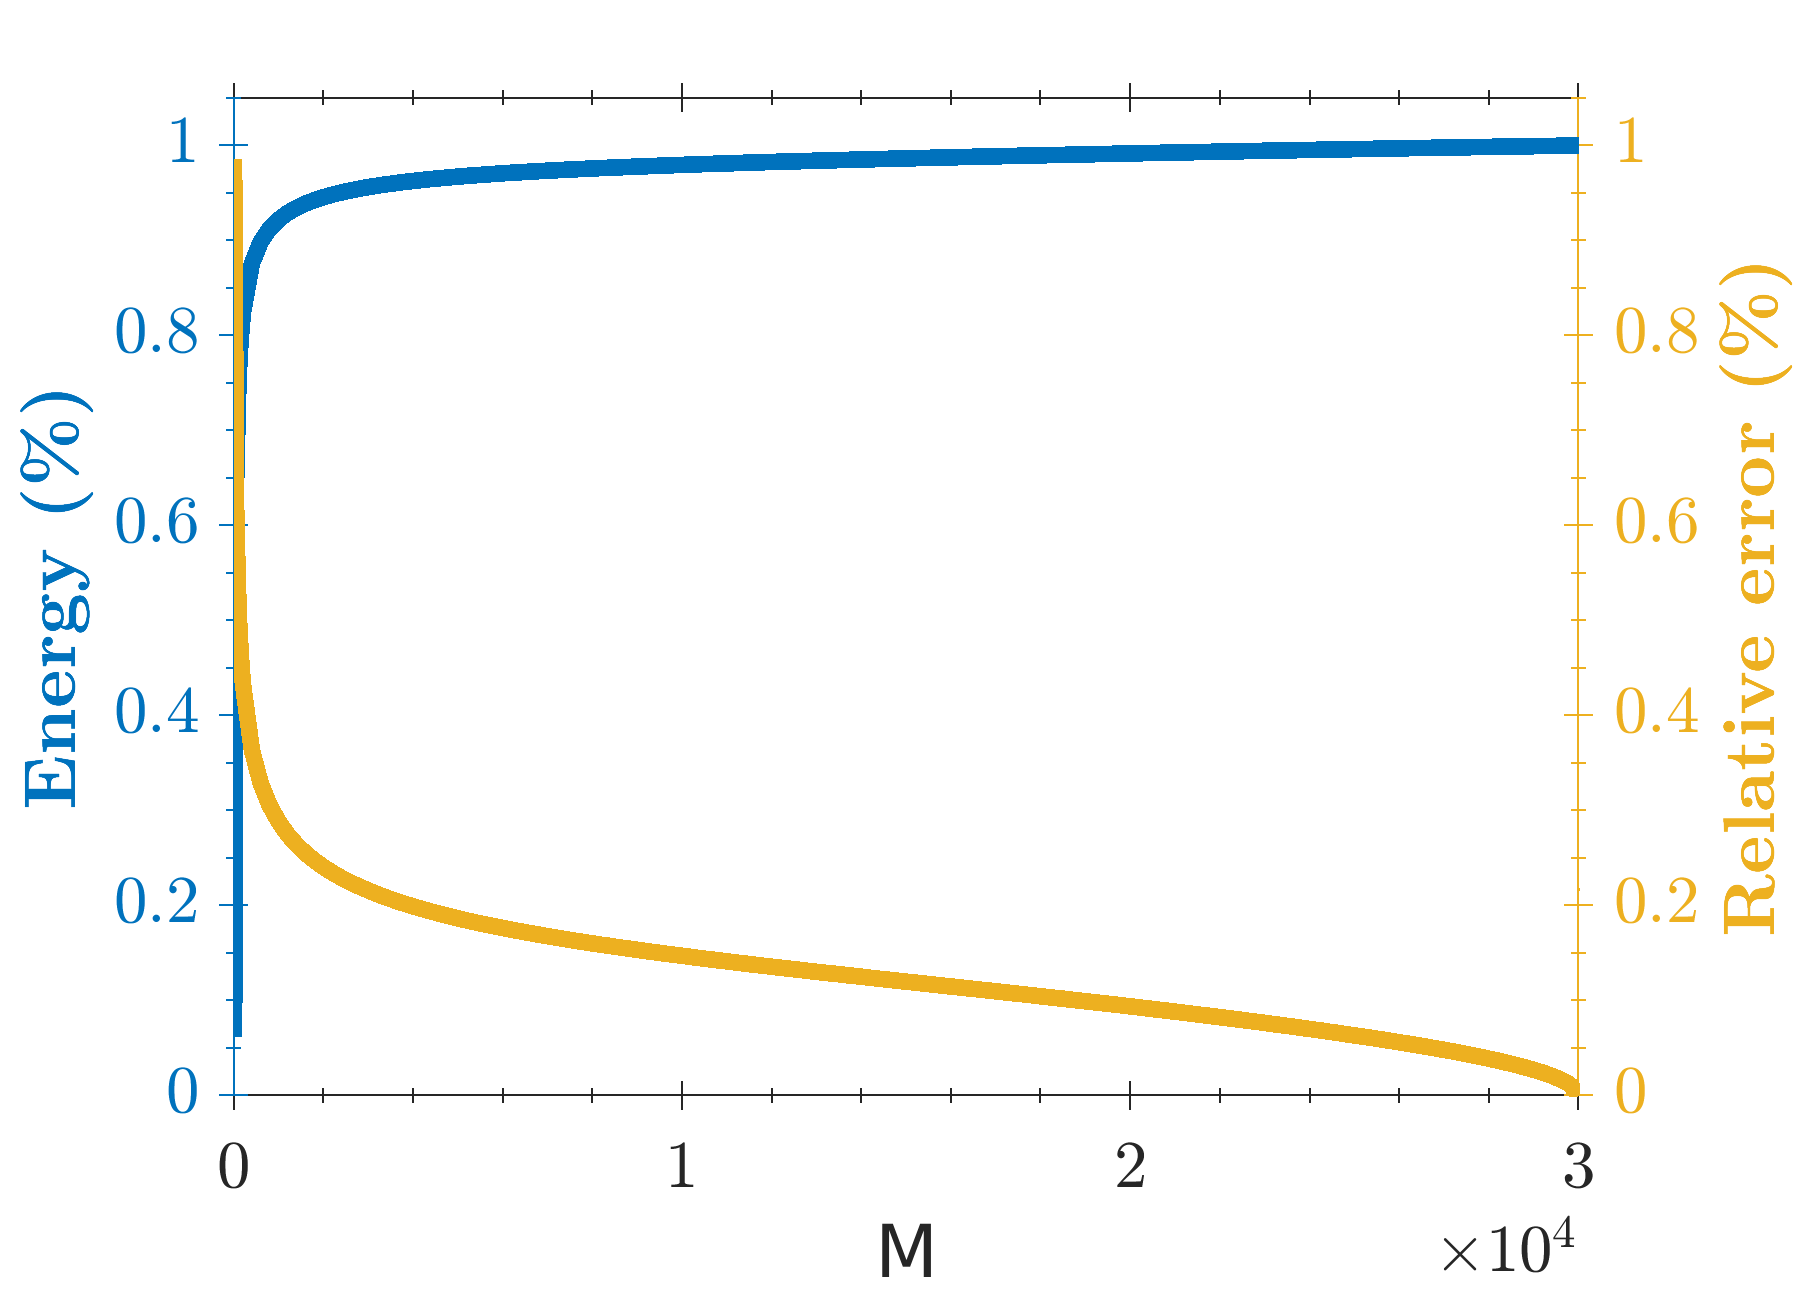
\includegraphics[scale=0.475]{./figuras/Energy_exp_100x100x1_0-2x0-2_30000.png}
 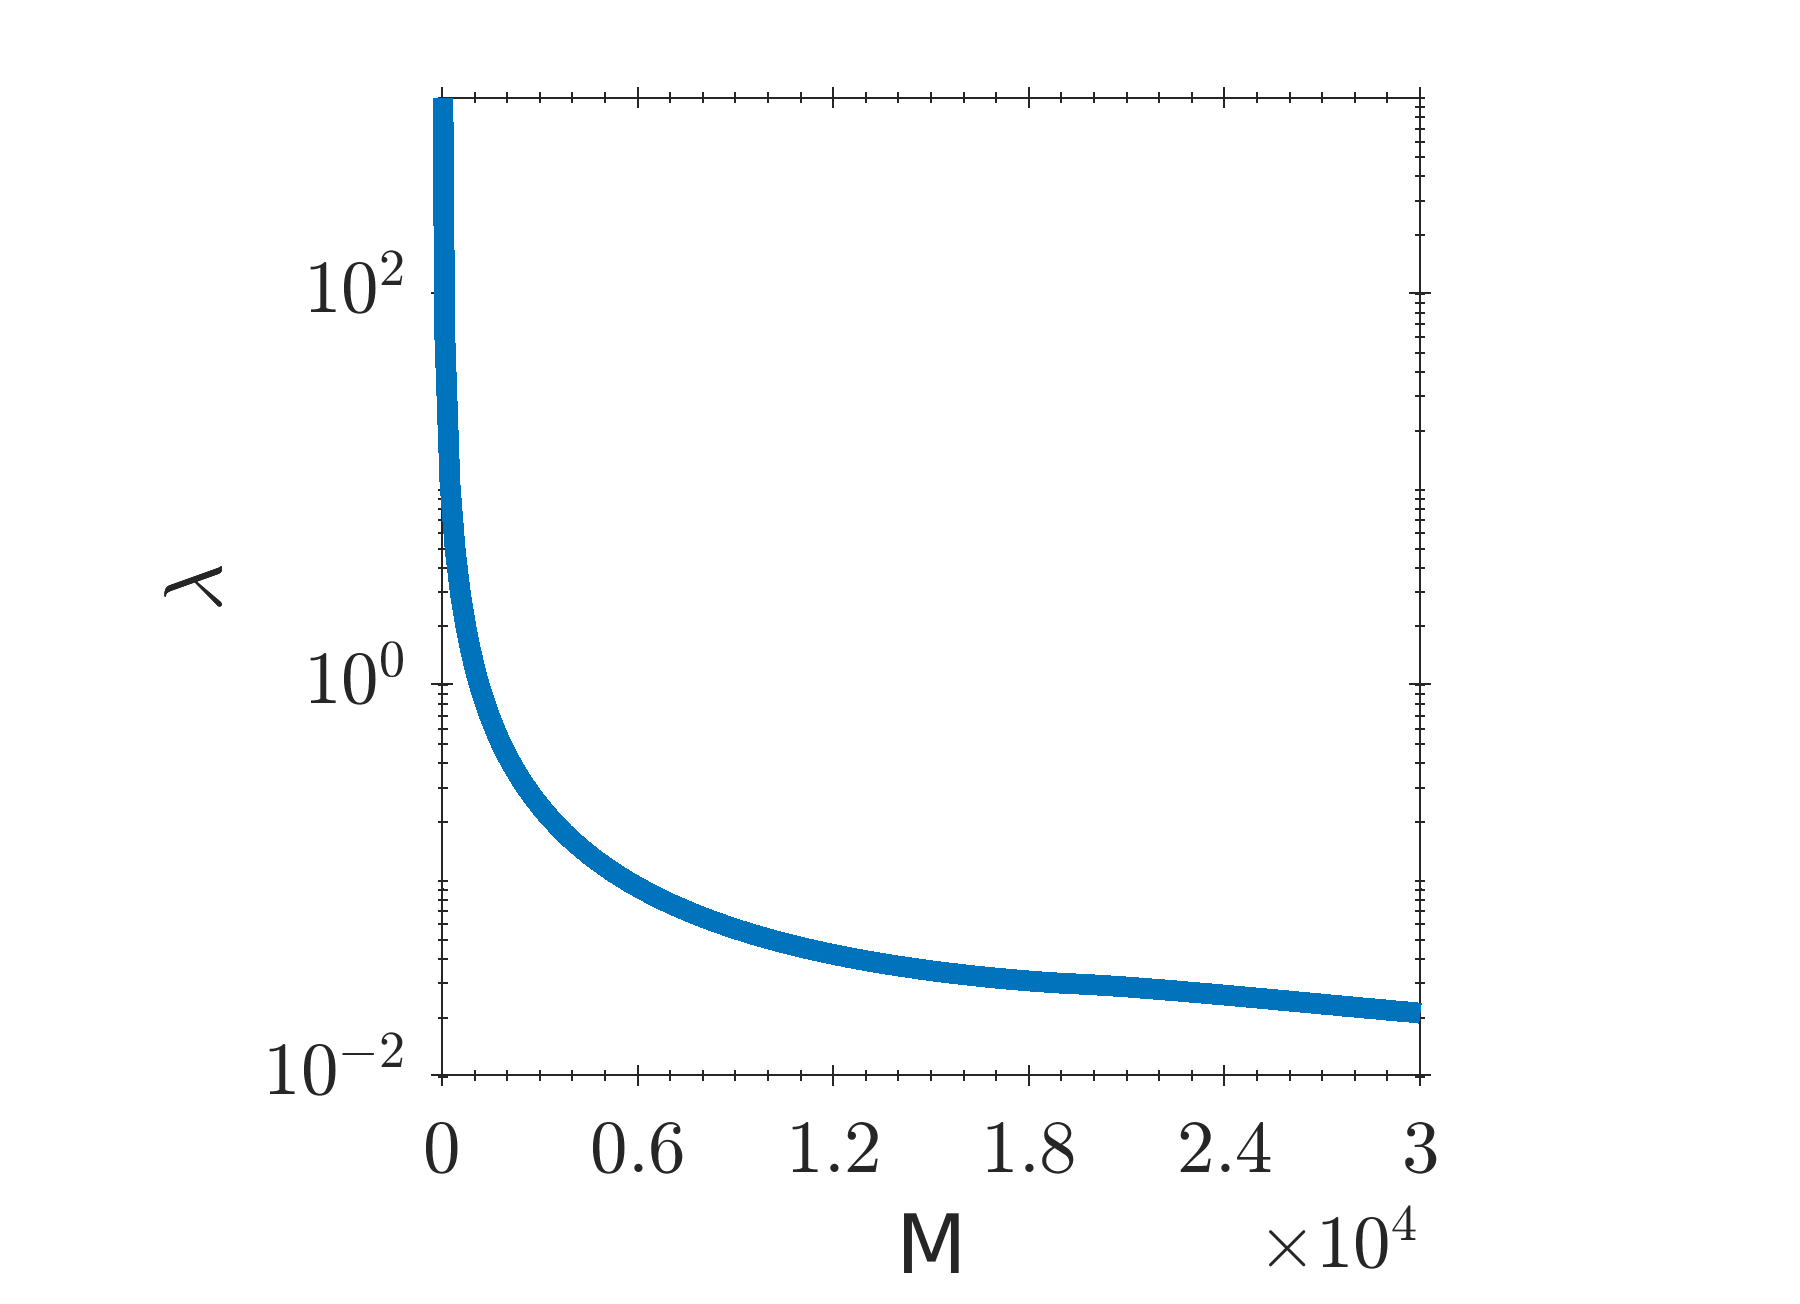
\includegraphics[scale=0.485]{./figuras/exp_autoval_100x100x1_0-2x0-2_30000.png}}
 \caption{Decay of eigenvalues and contained energy as a function of the number of terms in the expansion.}
 \label{eigenvalues}
\end{figure}


%%%%%%%%%%%%%%%%%%%%%%%%%%%%%%%%%%%%%%%%%%%%%%%%%%%%%%%%%%%%%%%%%%%%%%%%%%%%%%%%%%%%%%
\begin{figure}[H]
 \centering
 \subfigure[$\En=80\%$]{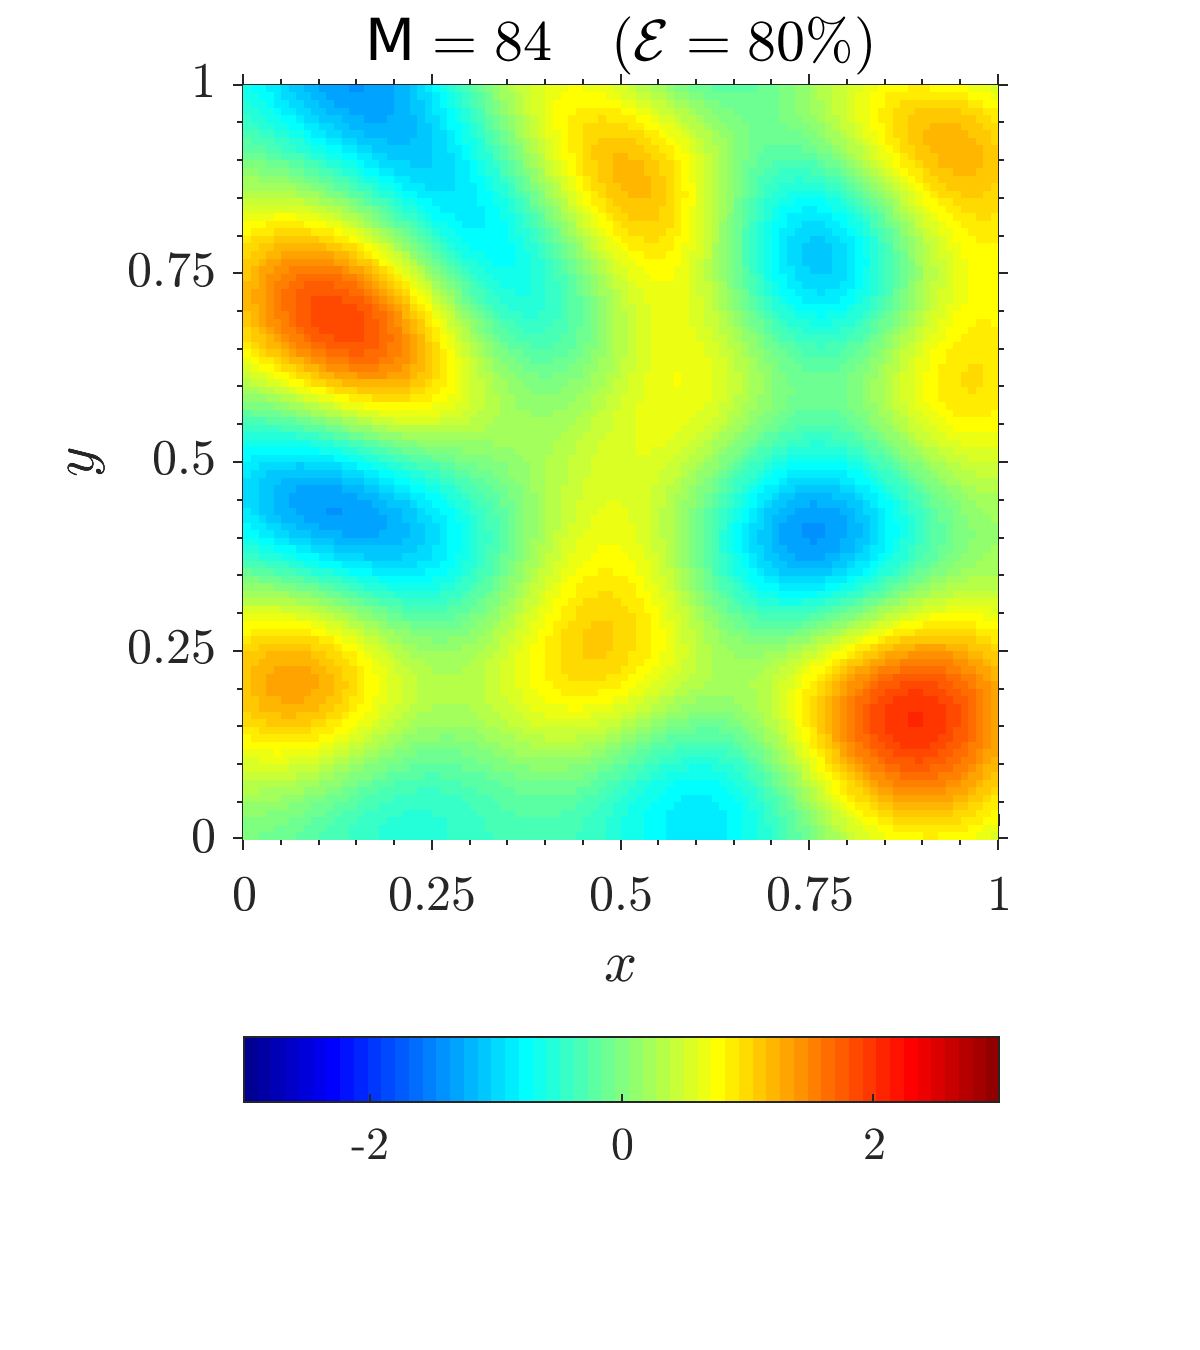
\includegraphics[scale=0.5]{figuras/Y_sexp_01_E80.png}
 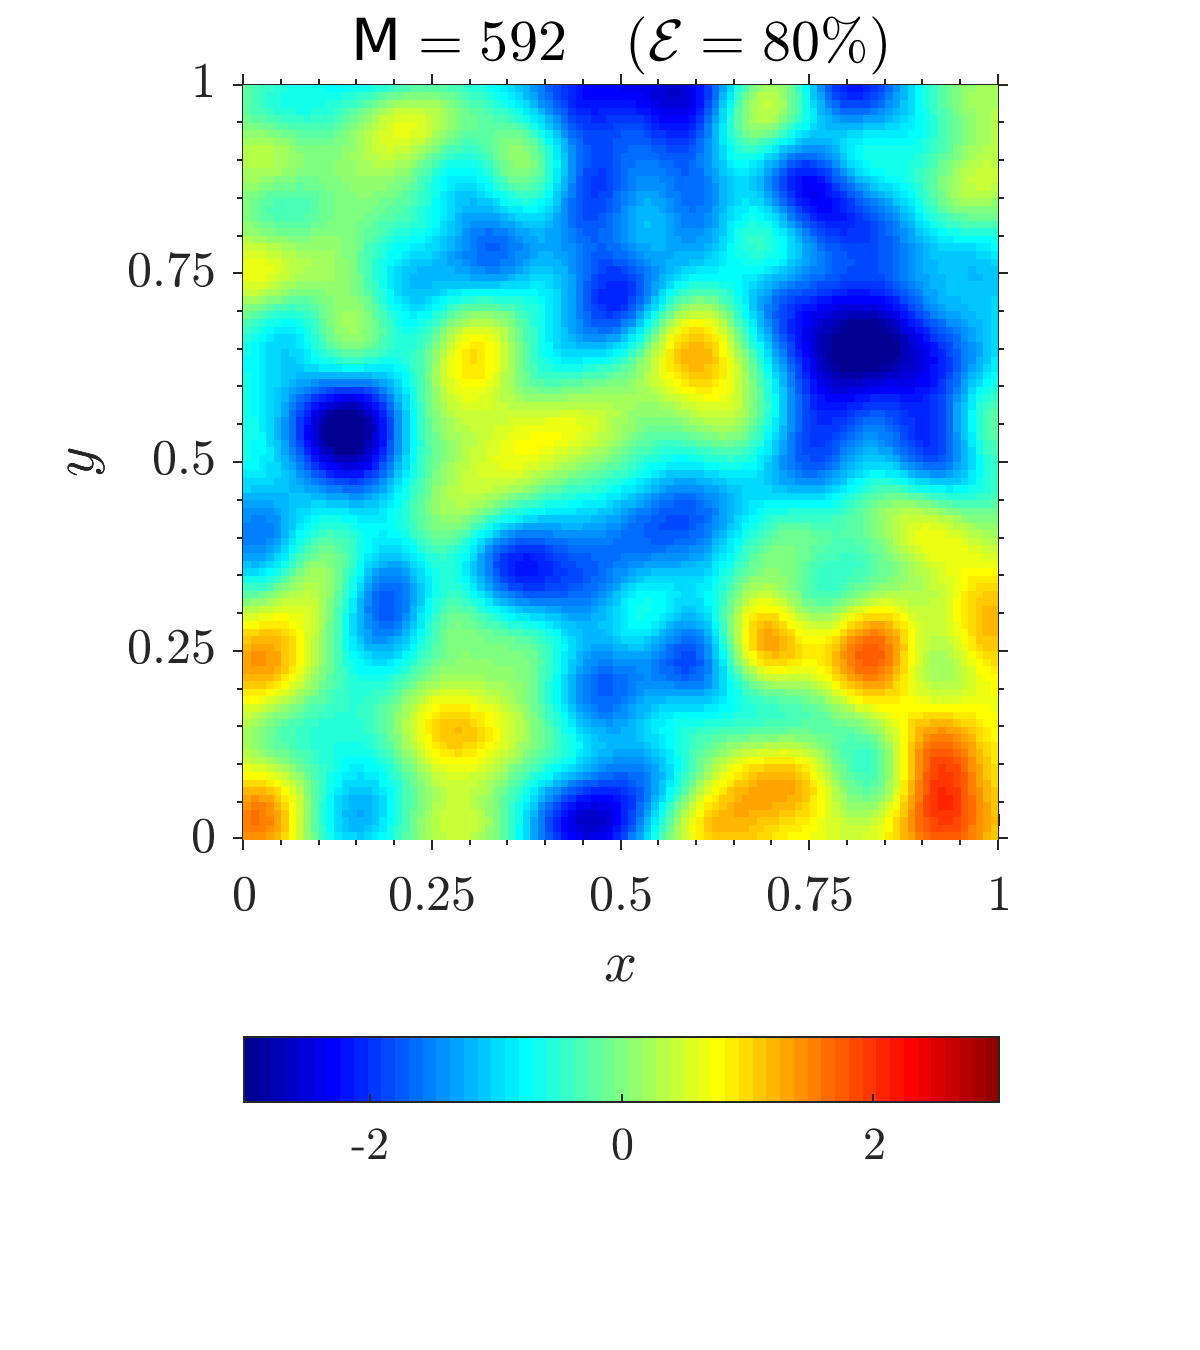
\includegraphics[scale=0.5]{figuras/Y_exp_01_E80.png}
 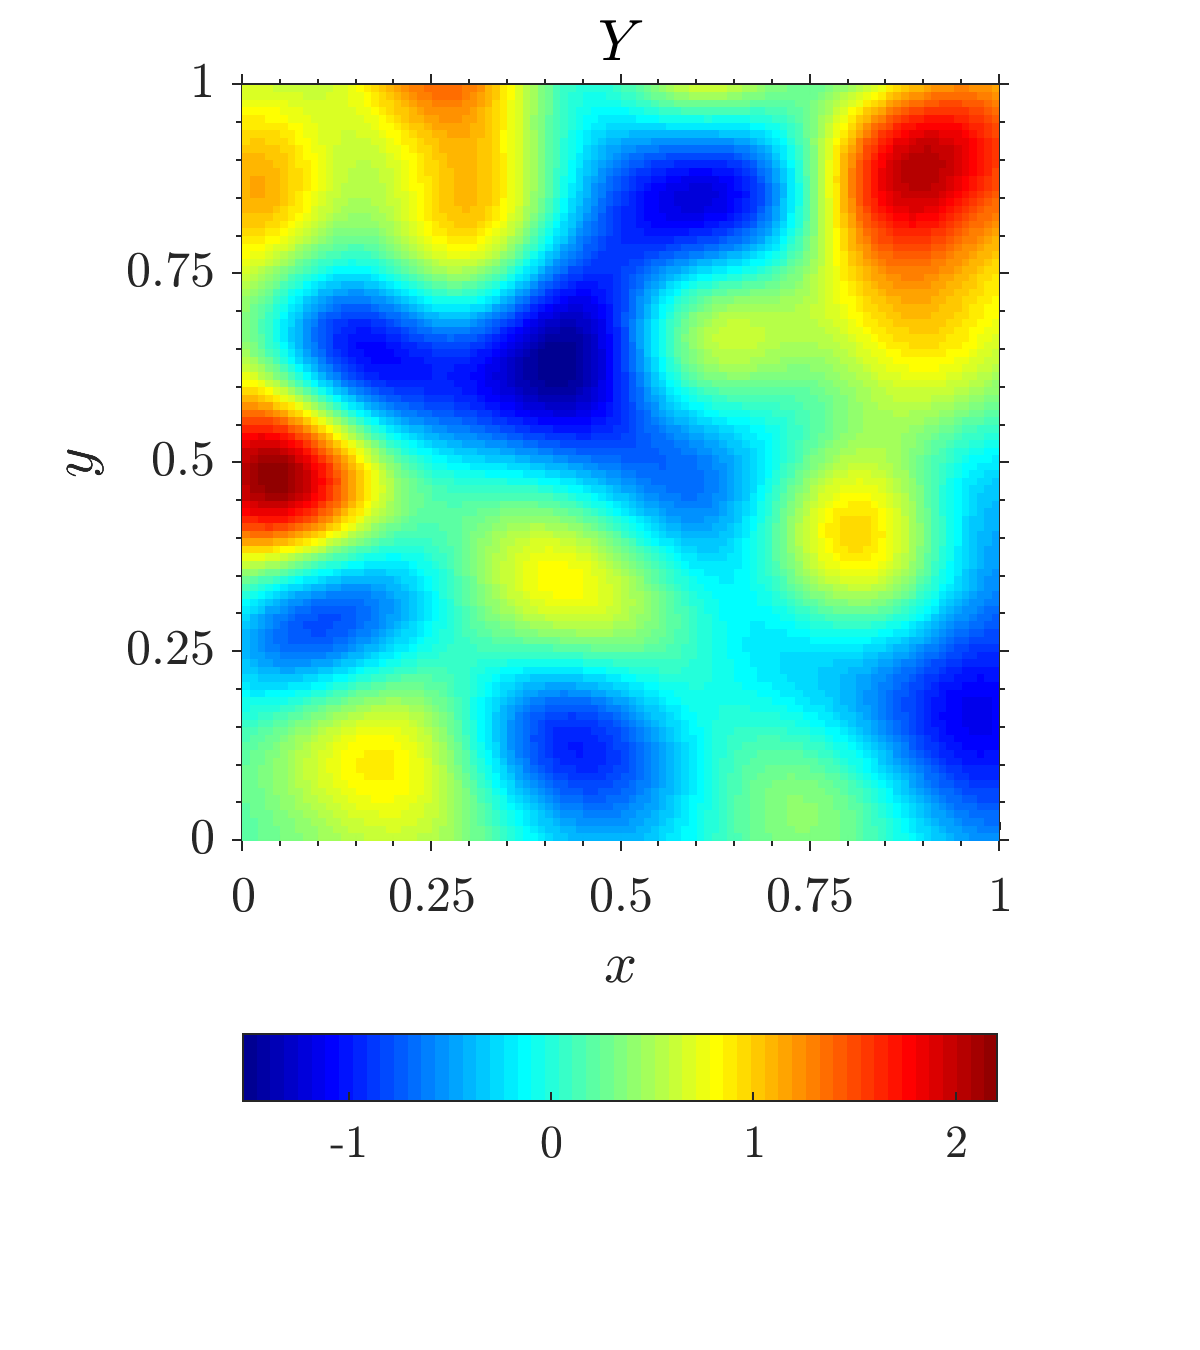
\includegraphics[scale=0.5]{figuras/Y_exp_02_E80.png}}
 \subfigure[$\En=96\%$]{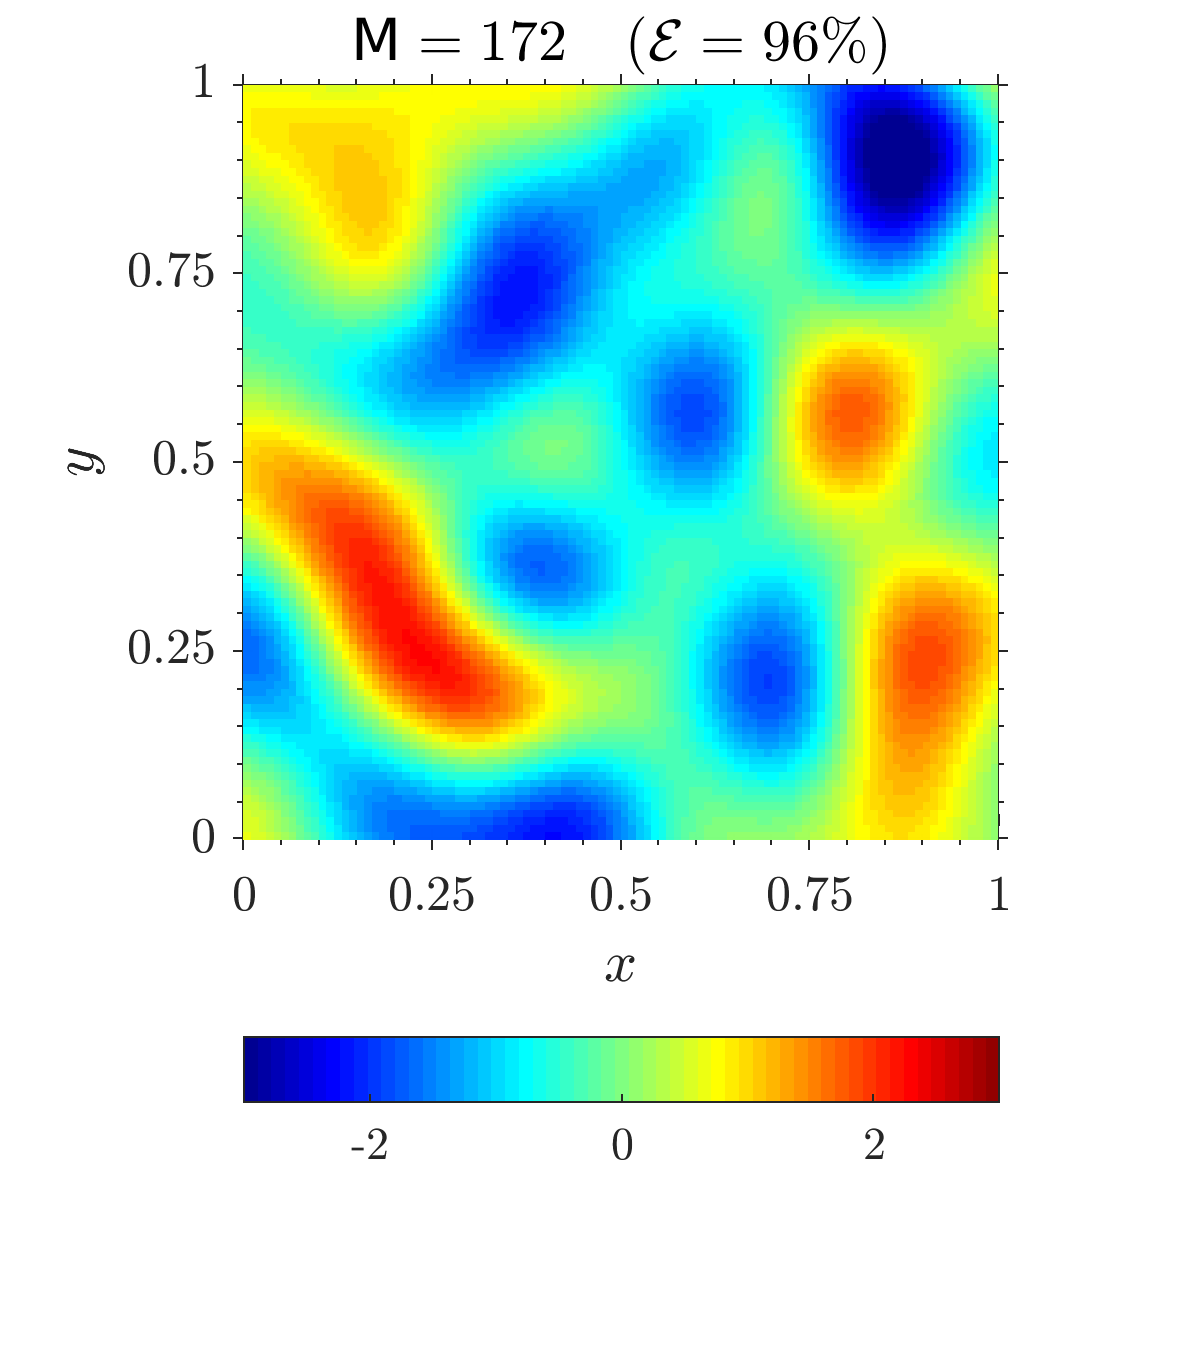
\includegraphics[scale=0.5]{figuras/Y_sexp_01_E96.png}
 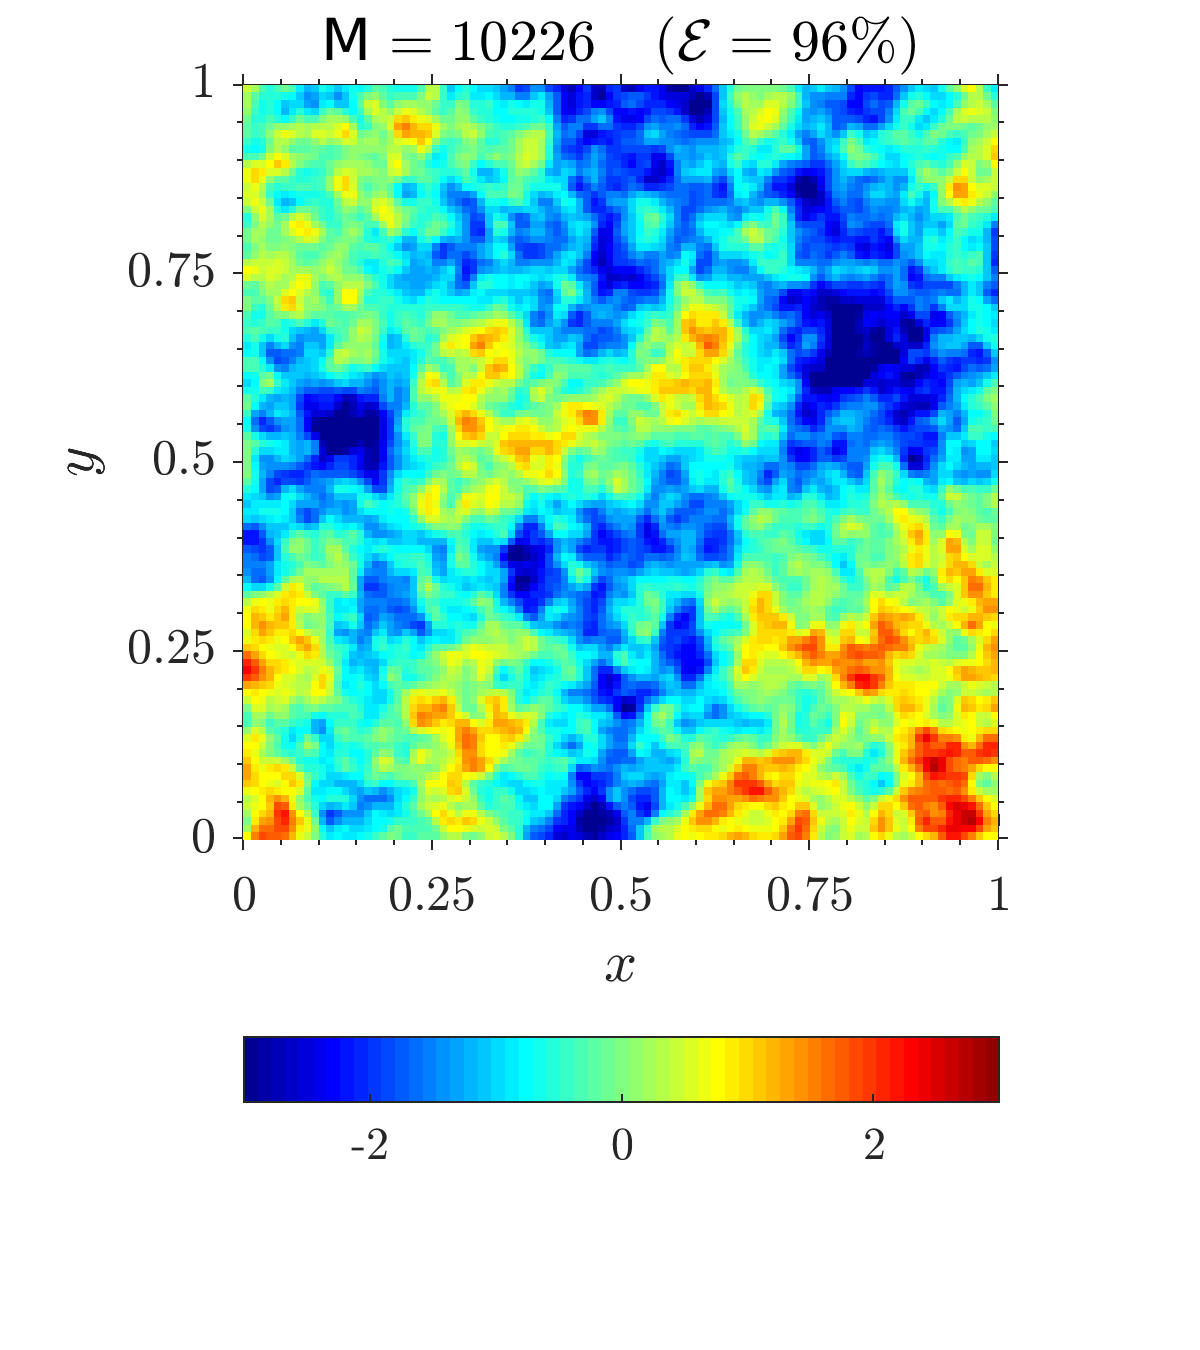
\includegraphics[scale=0.5]{figuras/Y_exp_01_E96.png}
 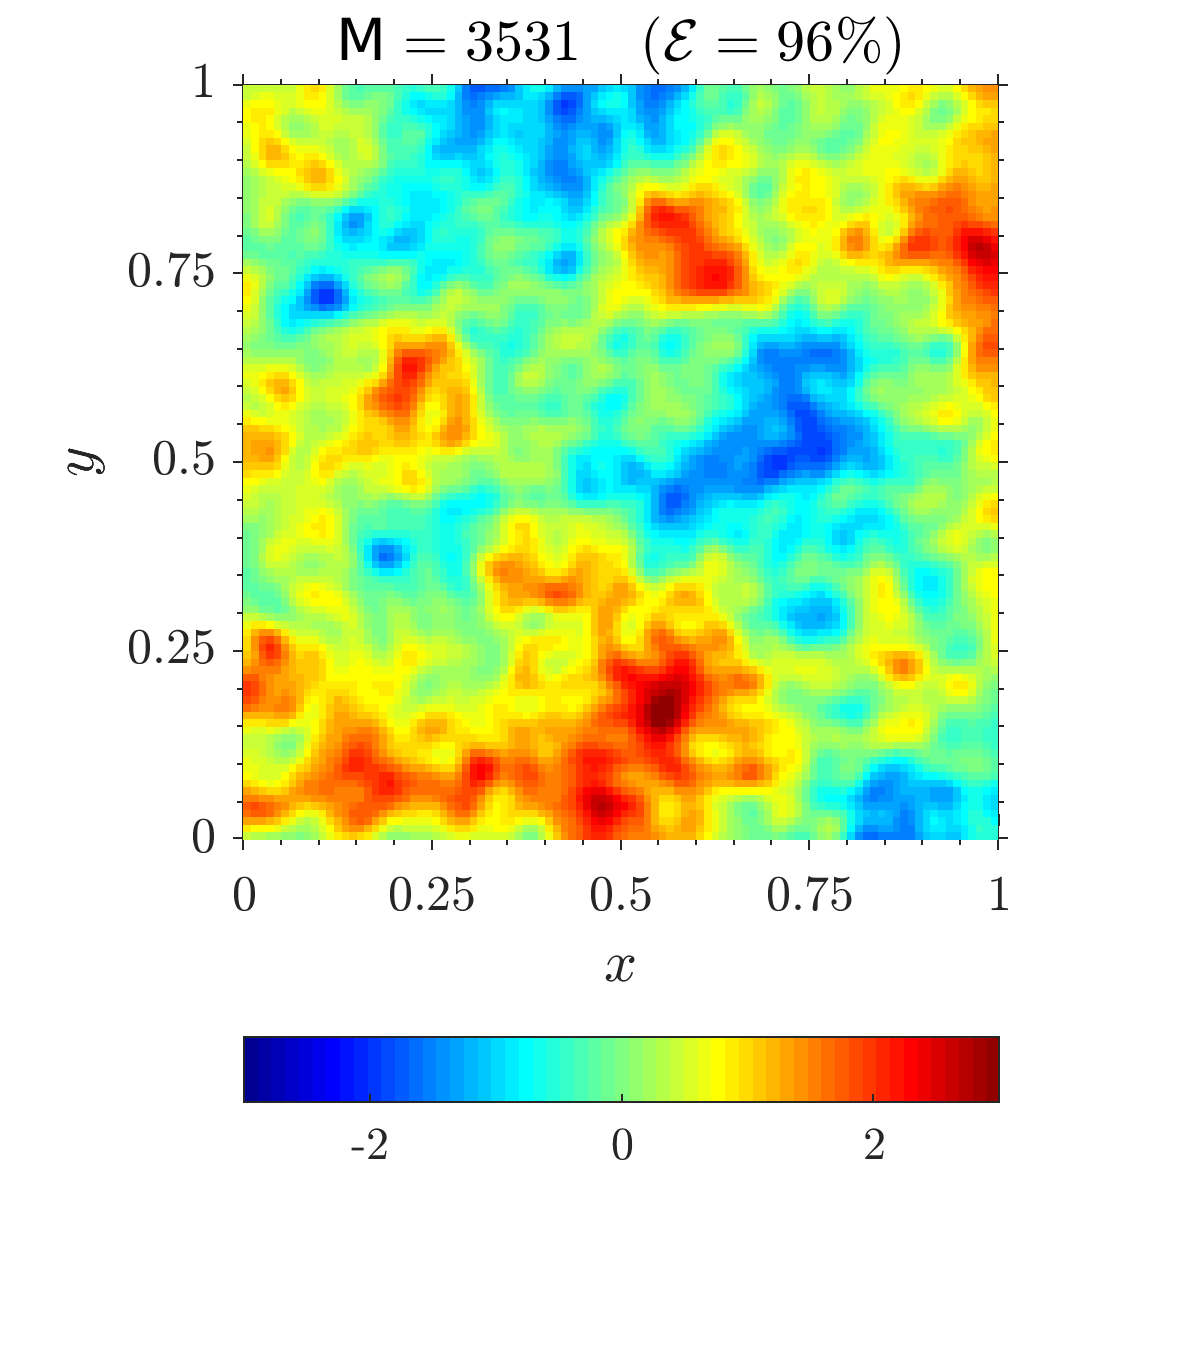
\includegraphics[scale=0.5]{figuras/Y_exp_02_E96.png}}
 \subfigure[$\En\sim 100\%$]{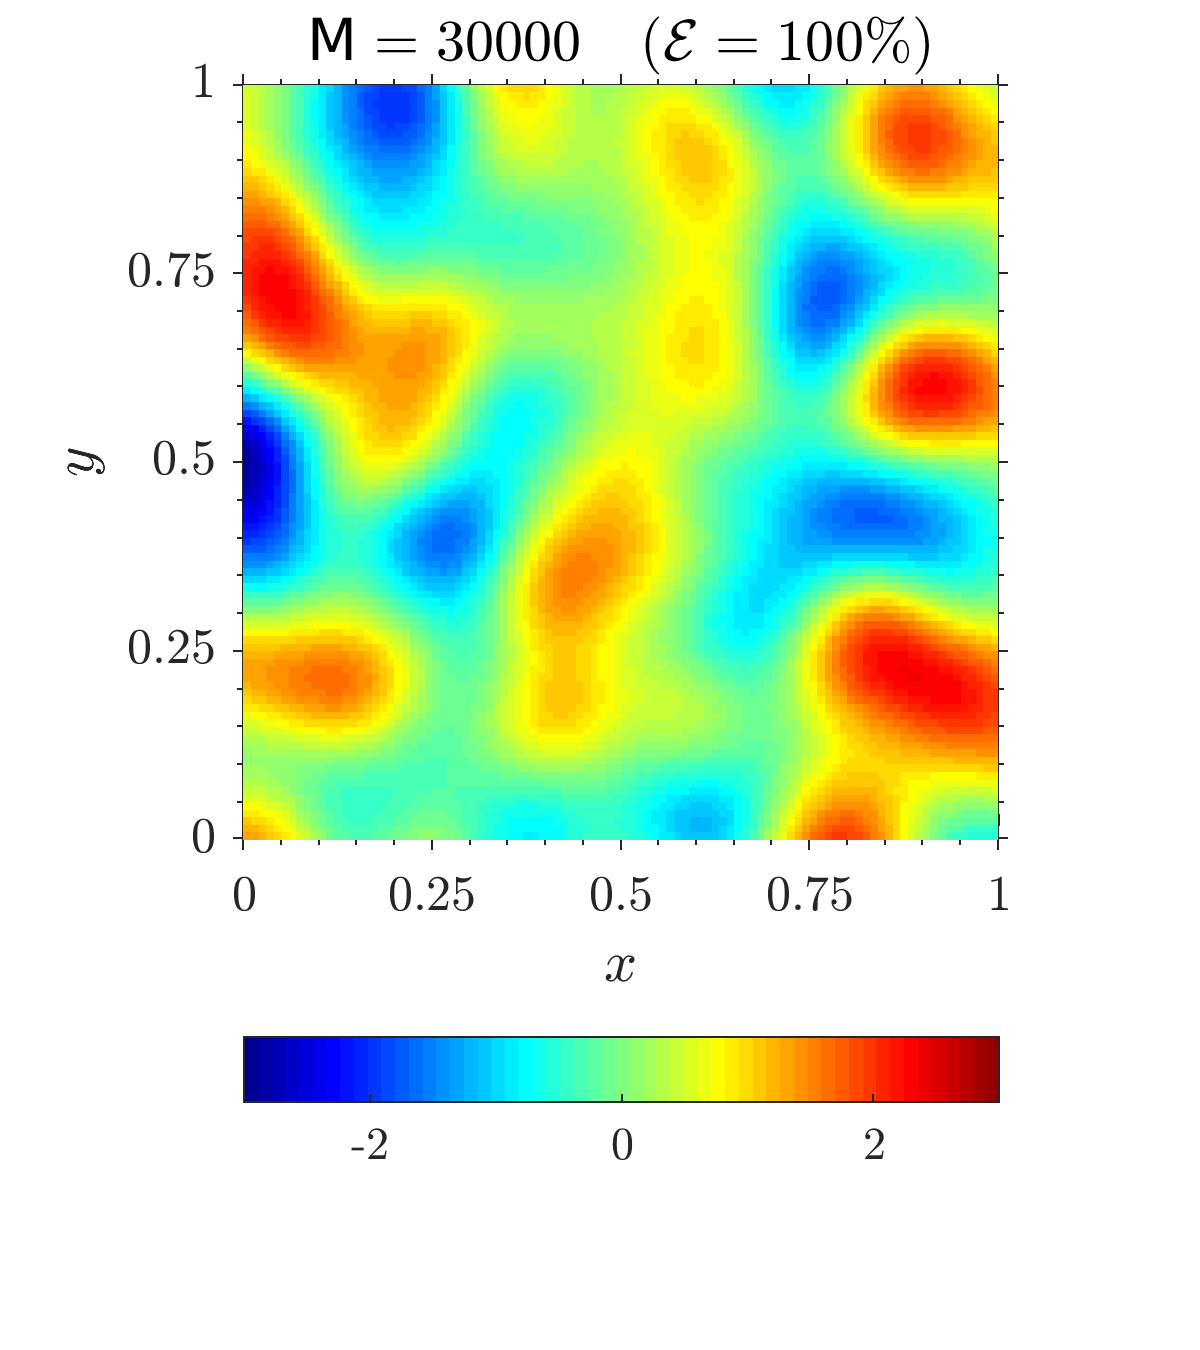
\includegraphics[scale=0.5]{figuras/Y_sexp_01_E100.png}
 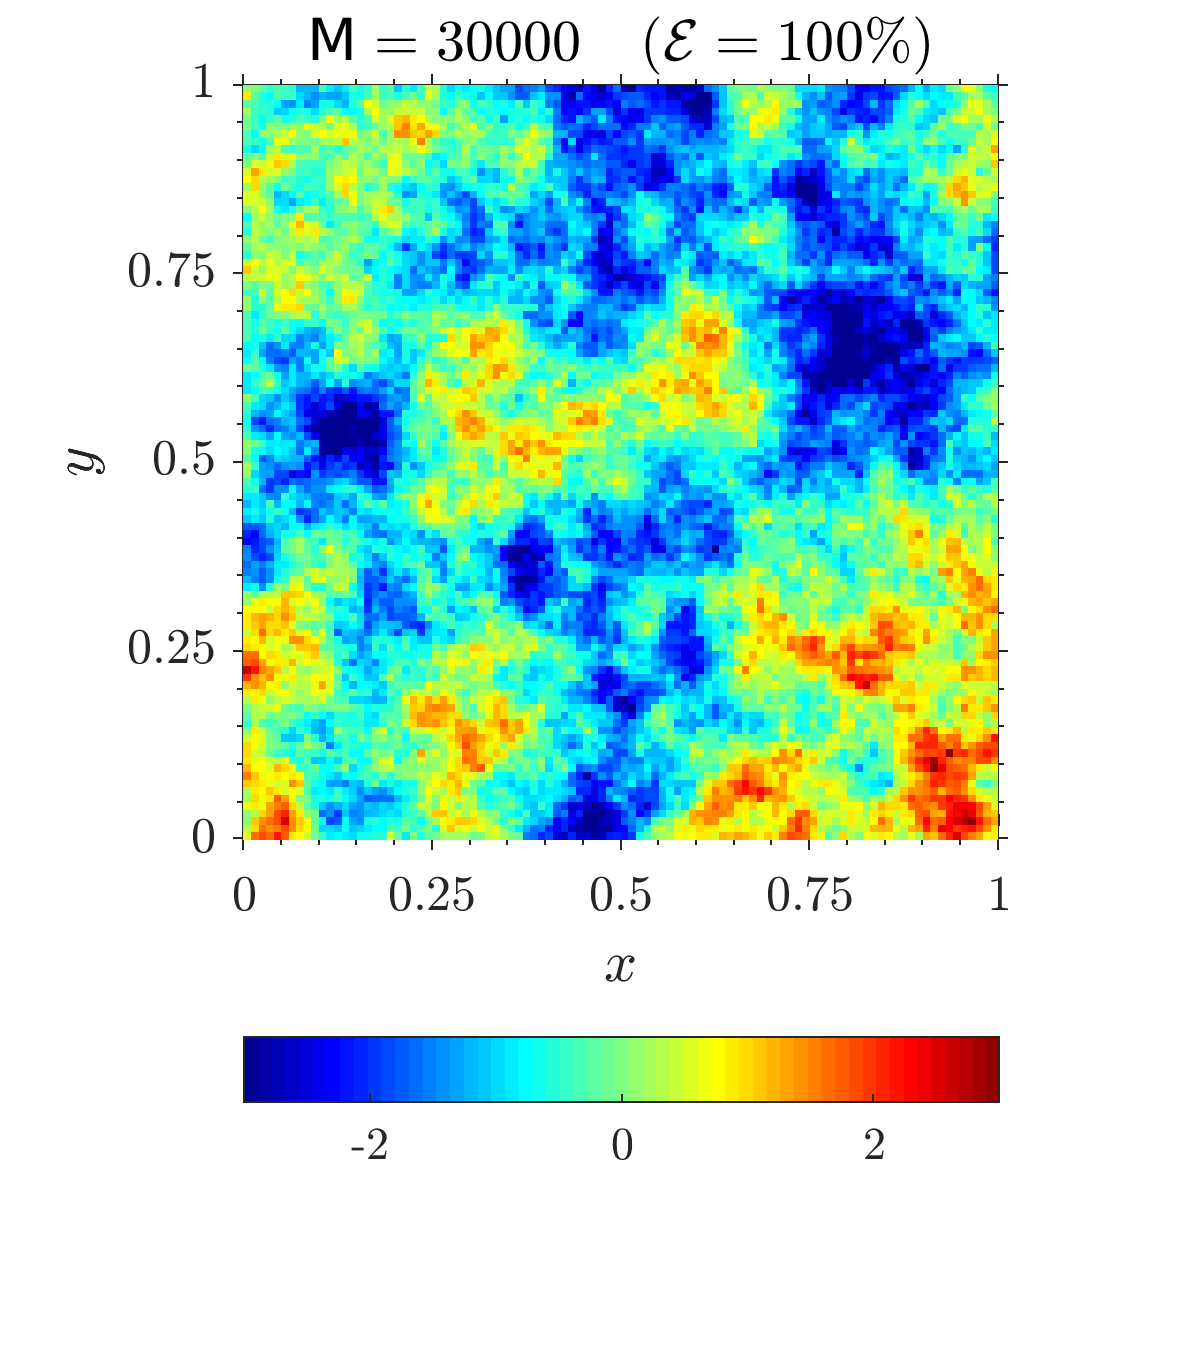
\includegraphics[scale=0.5]{figuras/Y_exp_01_E100.png}
 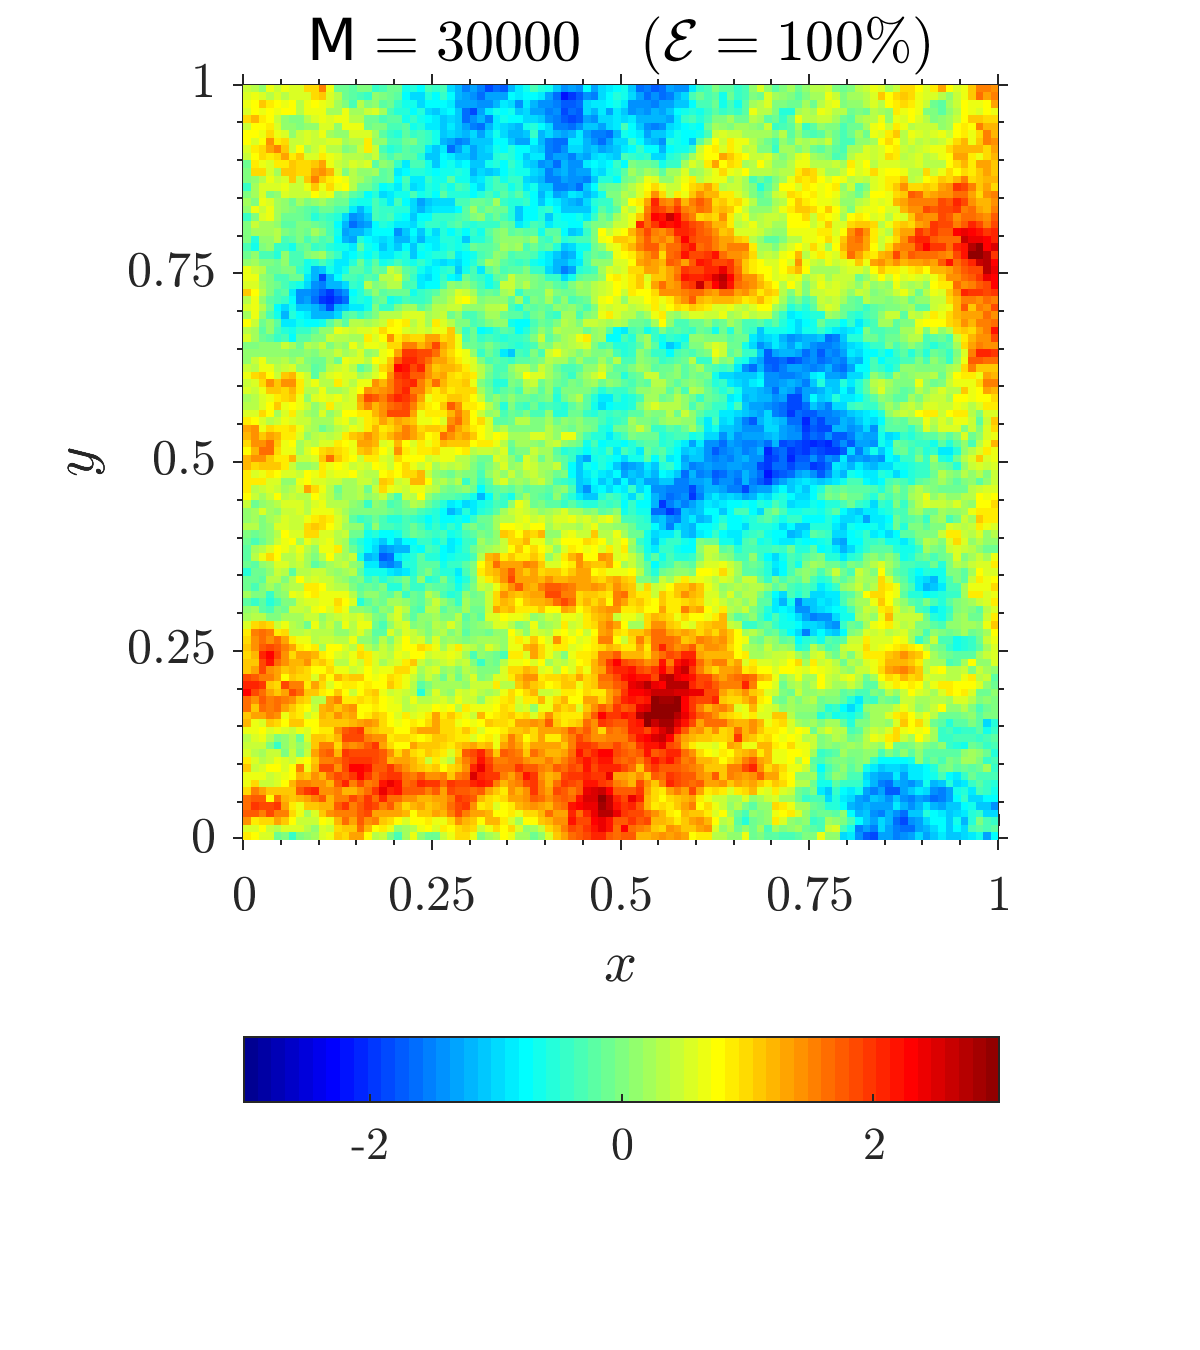
\includegraphics[scale=0.5]{figuras/Y_exp_02_E100.png}}
\end{figure}

%%%%%%%%%%%%%%%%%%%%%%%%%%%%%%%%%%%%%%%%%%%%%%%%%%%%%%%%%%%%%%%%%%%%%%%%%%%%%%%%%%%%%%
{\small
\begin{table}[H]
\caption{Number of \kl\ expansion terms needed to obtain an given energy level}
\label{tab:KLE}
{
\newcommand{\mc}[3]{\multicolumn{#1}{#2}{#3}}
\begin{center}
\begin{tabular}{lccc|ccc}\hline\hline
\cline{1-7}
\mc{1}{l|}{\textbf{Energy}} & \mc{3}{c|}{$\m$} & \mc{3}{c}{\textbf{Mean relative error}}\\\cline{2-7}
\mc{1}{l|}{\textbf{}} & Squared Exp. & Exponential & Exponential & Squared Exp. & Exponential & Exponential \\
\mc{1}{l|}{\textbf{($\%$)}} & ($\clen=0.1$) & ($\clen=0.1$) & ($\clen=0.2$) & ($\clen=0.1$) & ($\clen=0.1$) & ($\clen=0.2$)\\\hline
\mc{1}{l|}{\textbf{80}} & 84  & 592   & 154 & 0.46 & 0.45 & 0.47\\
\mc{1}{l|}{\textbf{90}} & 122 & 2,323  & 612 & 0.32 & 0.32 & 0.33\\
\mc{1}{l|}{\textbf{94}} & 150 & 5,760  & 1,655 & 0.25 & 0.25 & 0.25\\
\mc{1}{l|}{\textbf{96}} & 172 & 10,226 & 3,531 & 0.21 & 0.20 & 0.21\\
\mc{1}{l|}{\textbf{98}} & 211 & 18,327 & 10,239 & 0.14 & 0.14 & 0.15\\
\mc{1}{l|}{\textbf{100}}& $\sim$30,000 & $\sim$30,000 & $\sim$30,000 & 0.00 & 0.00 & 0.00\\\hline\hline
 \end{tabular}
 \end{center}
}
\end{table}
}
%%%%%%%%%%%%%%%%%%%%%%%%%%%%%%%%%%%%%%%%%%%%%%%%%%%%%%%%%%%%%%%%%%%%%%%%%%%%%%%%%%%%%%
\begin{figure}[H]
 \centering
 \subfigure[$x$ direction]{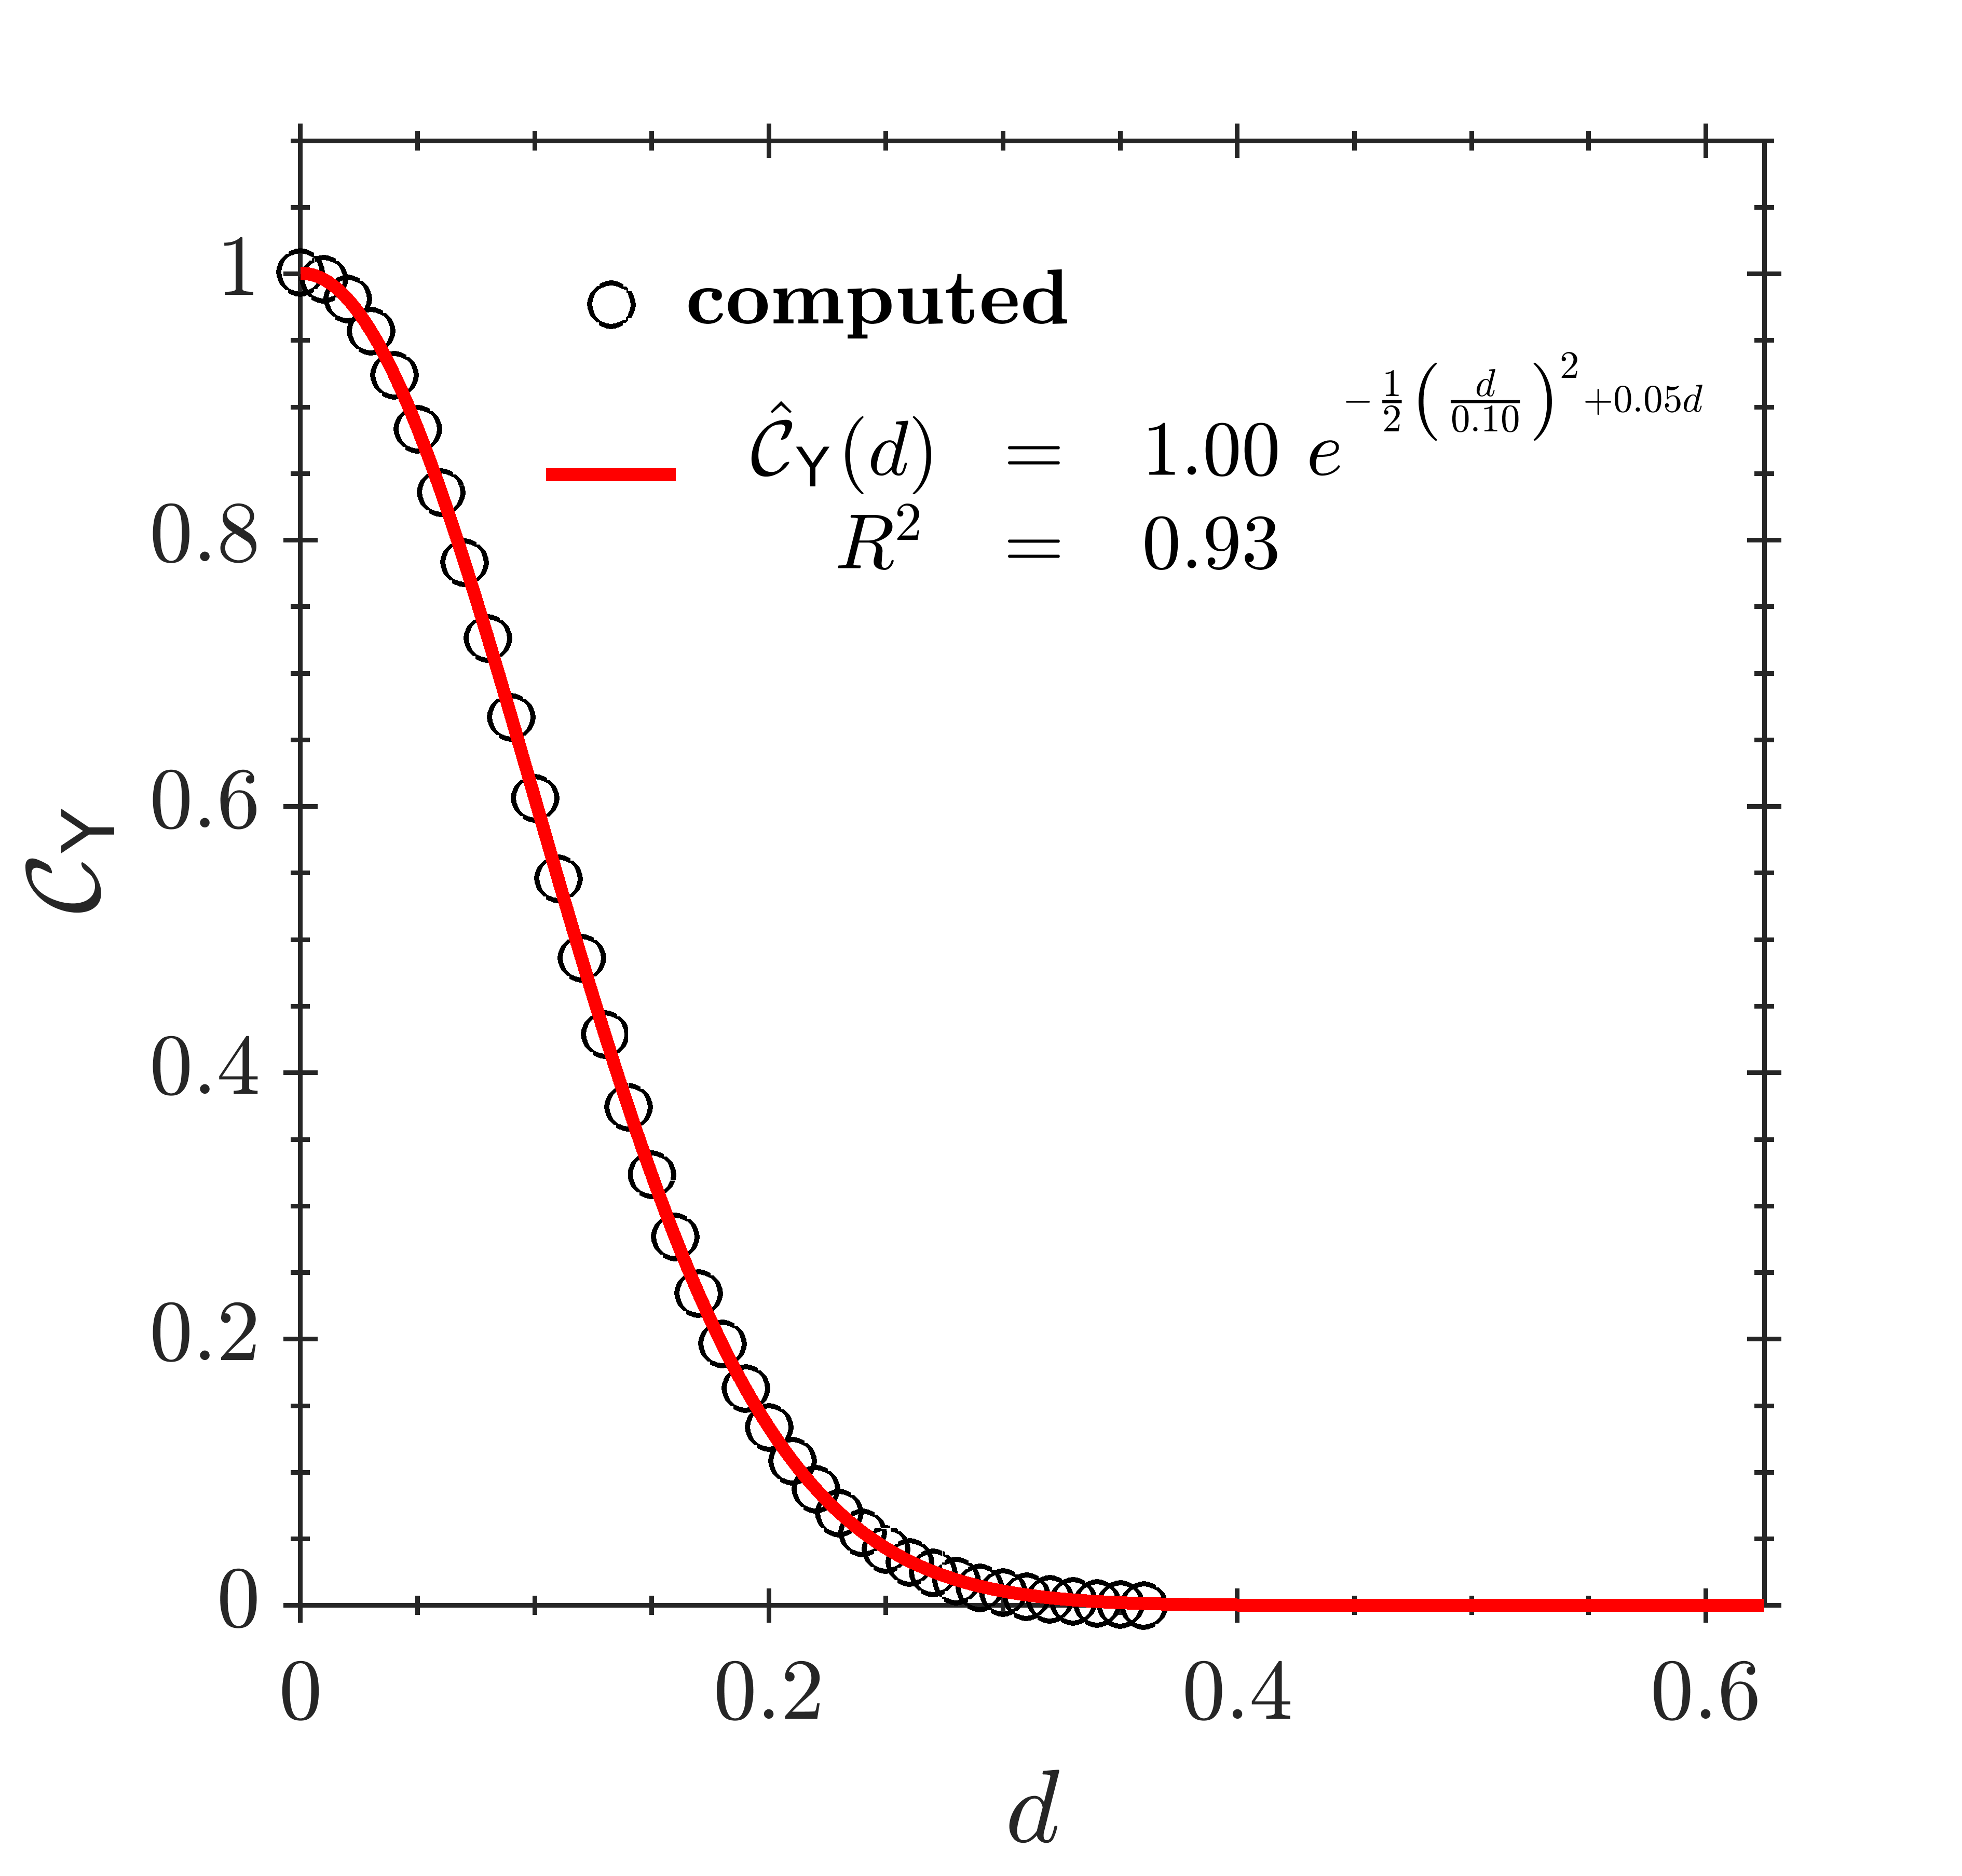
\includegraphics[scale=0.45]{./figuras/e_gssexp_1x1_100x100_0-1x0-1_5000_Yx.png}}
 \subfigure[$y$ direction]{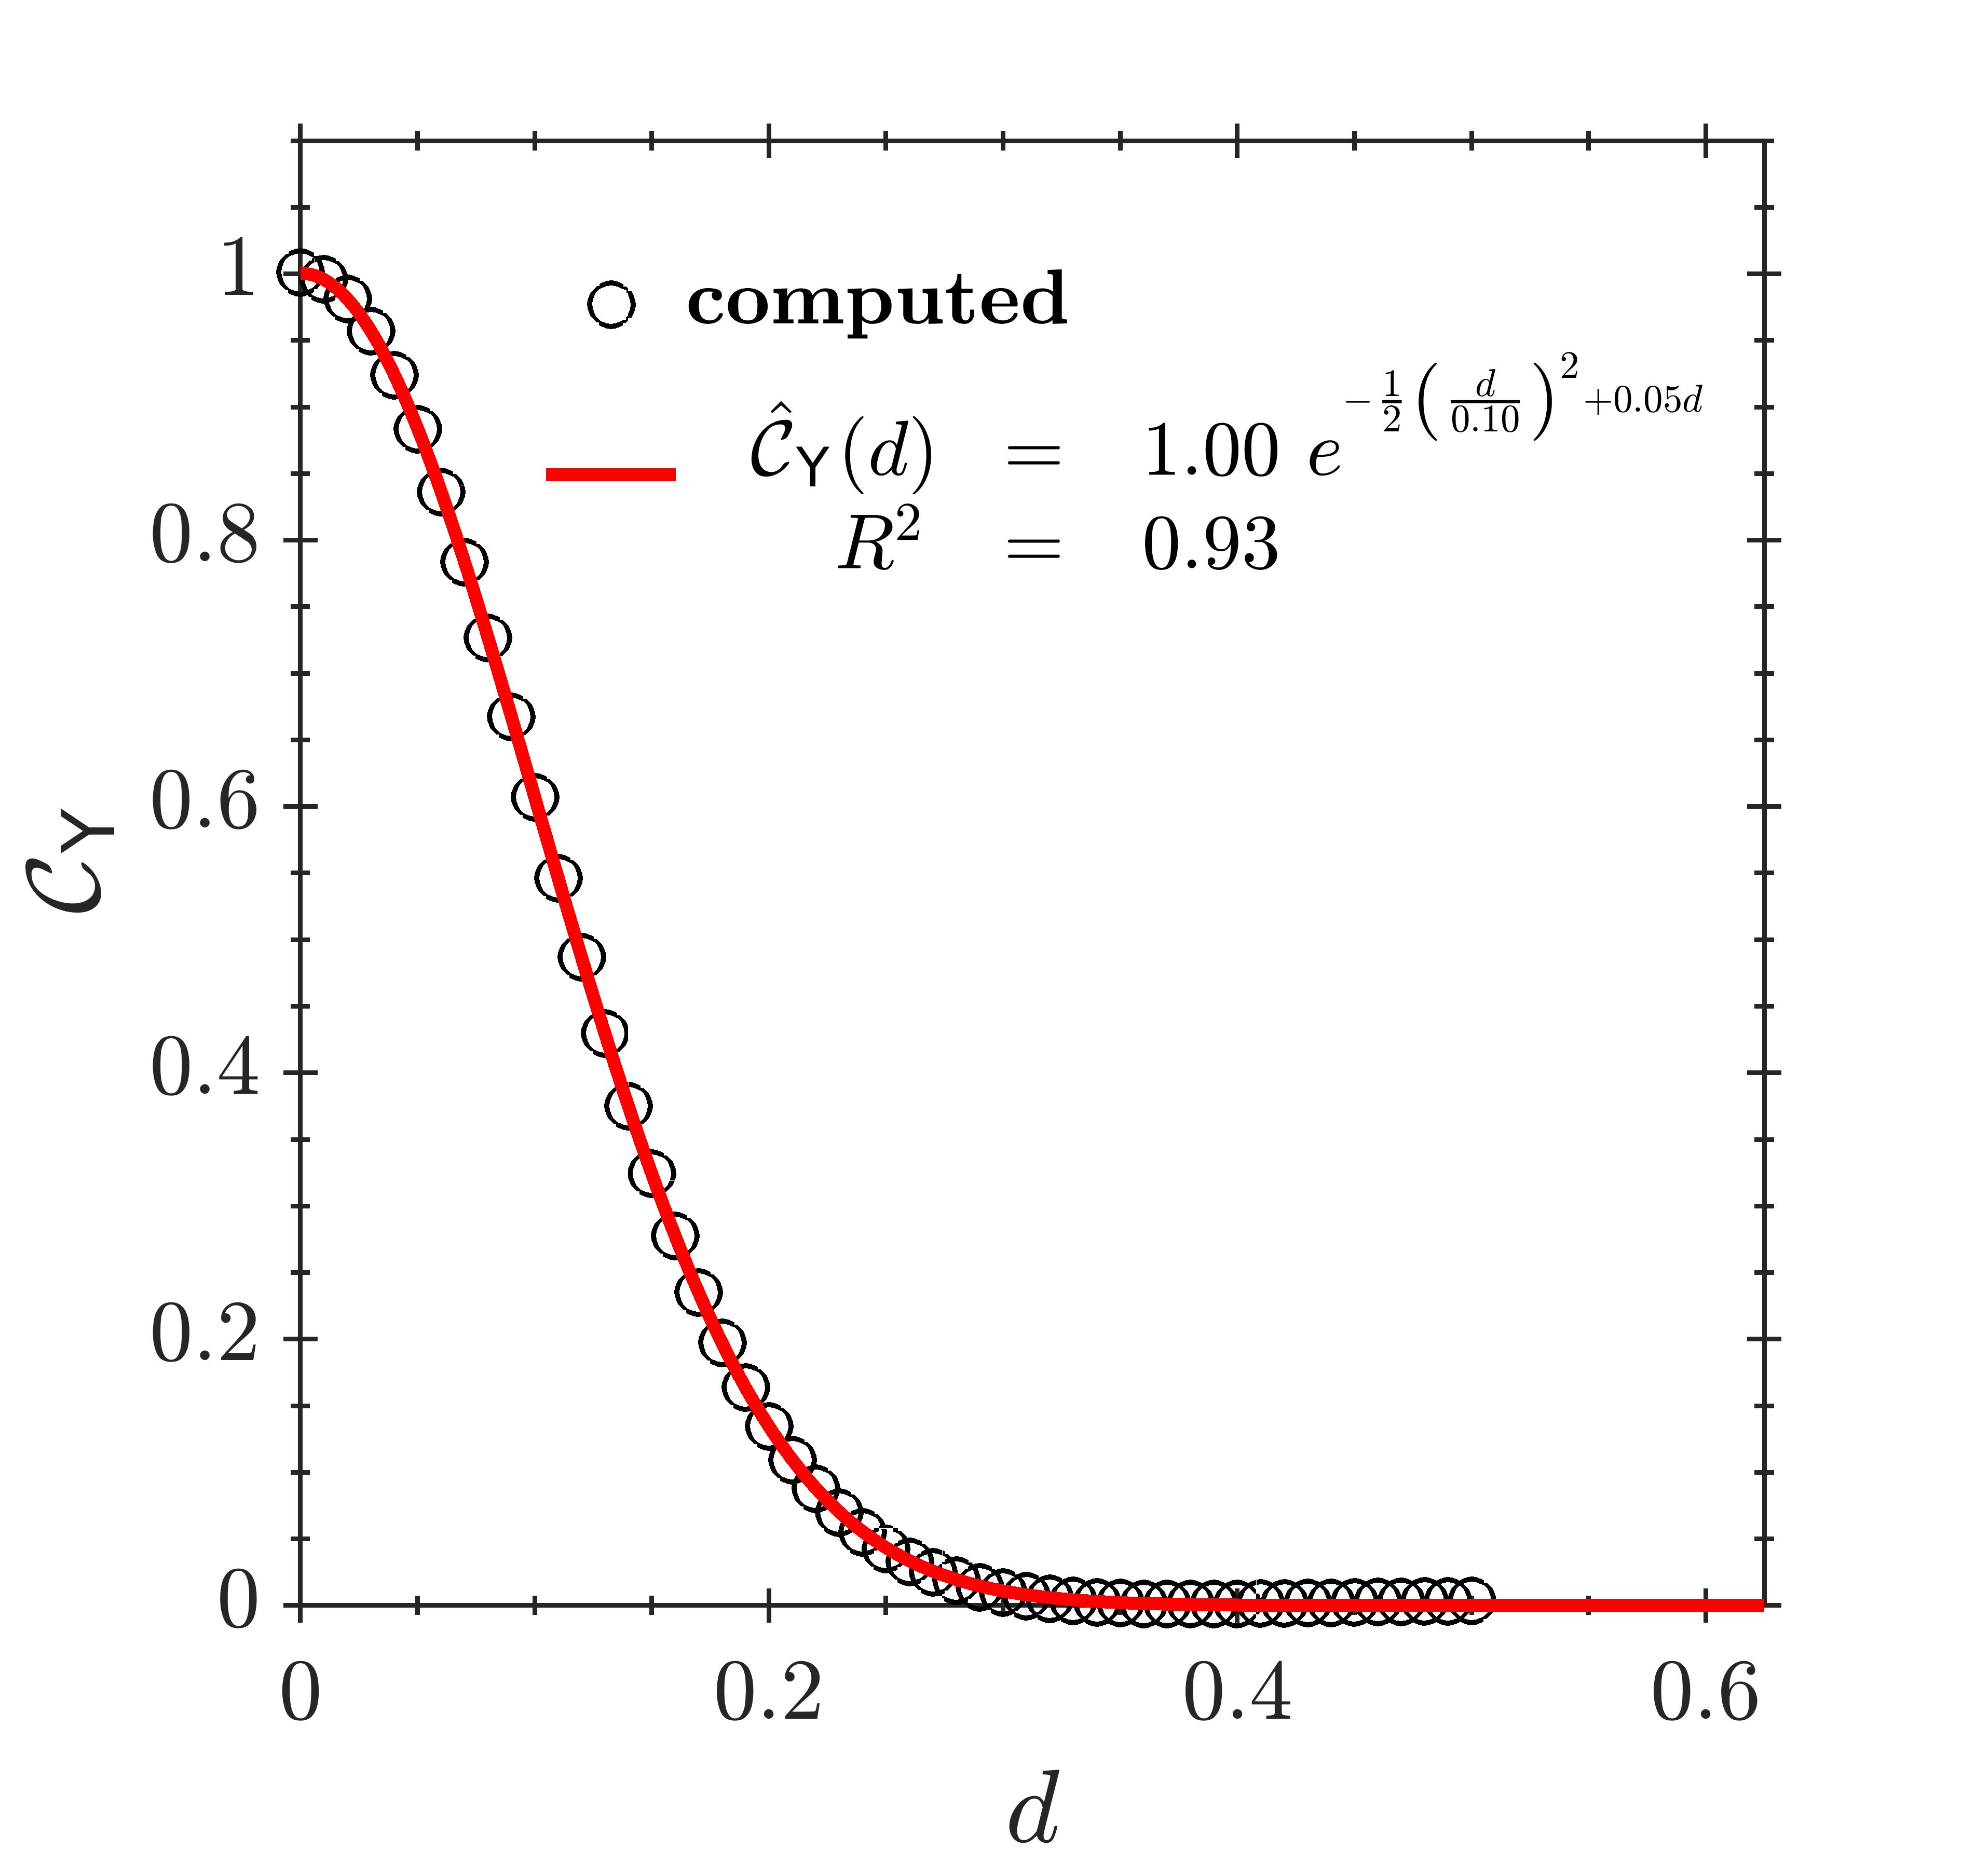
\includegraphics[scale=0.45]{./figuras/e_gssexp_1x1_100x100_0-1x0-1_5000_Yy.png}}
 \caption{Estimated covariance in a sample of $5,000$ fields generate by \kle\ with $30,000$ terms. Squared exponential case with $\clen = 0.1$.}
 \label{covar_sexpKL}
\end{figure}
%%%%%%%%%%%%%%%%%%%%%%%%%%%%%%%%%%%%%%%%%%%%%%%%%%%%%%%%%%%%%%%%%%%%%%%%%%%%%%%%%%%%%%
\begin{figure}[H]
 \centering
 \subfigure[$x$ direction]{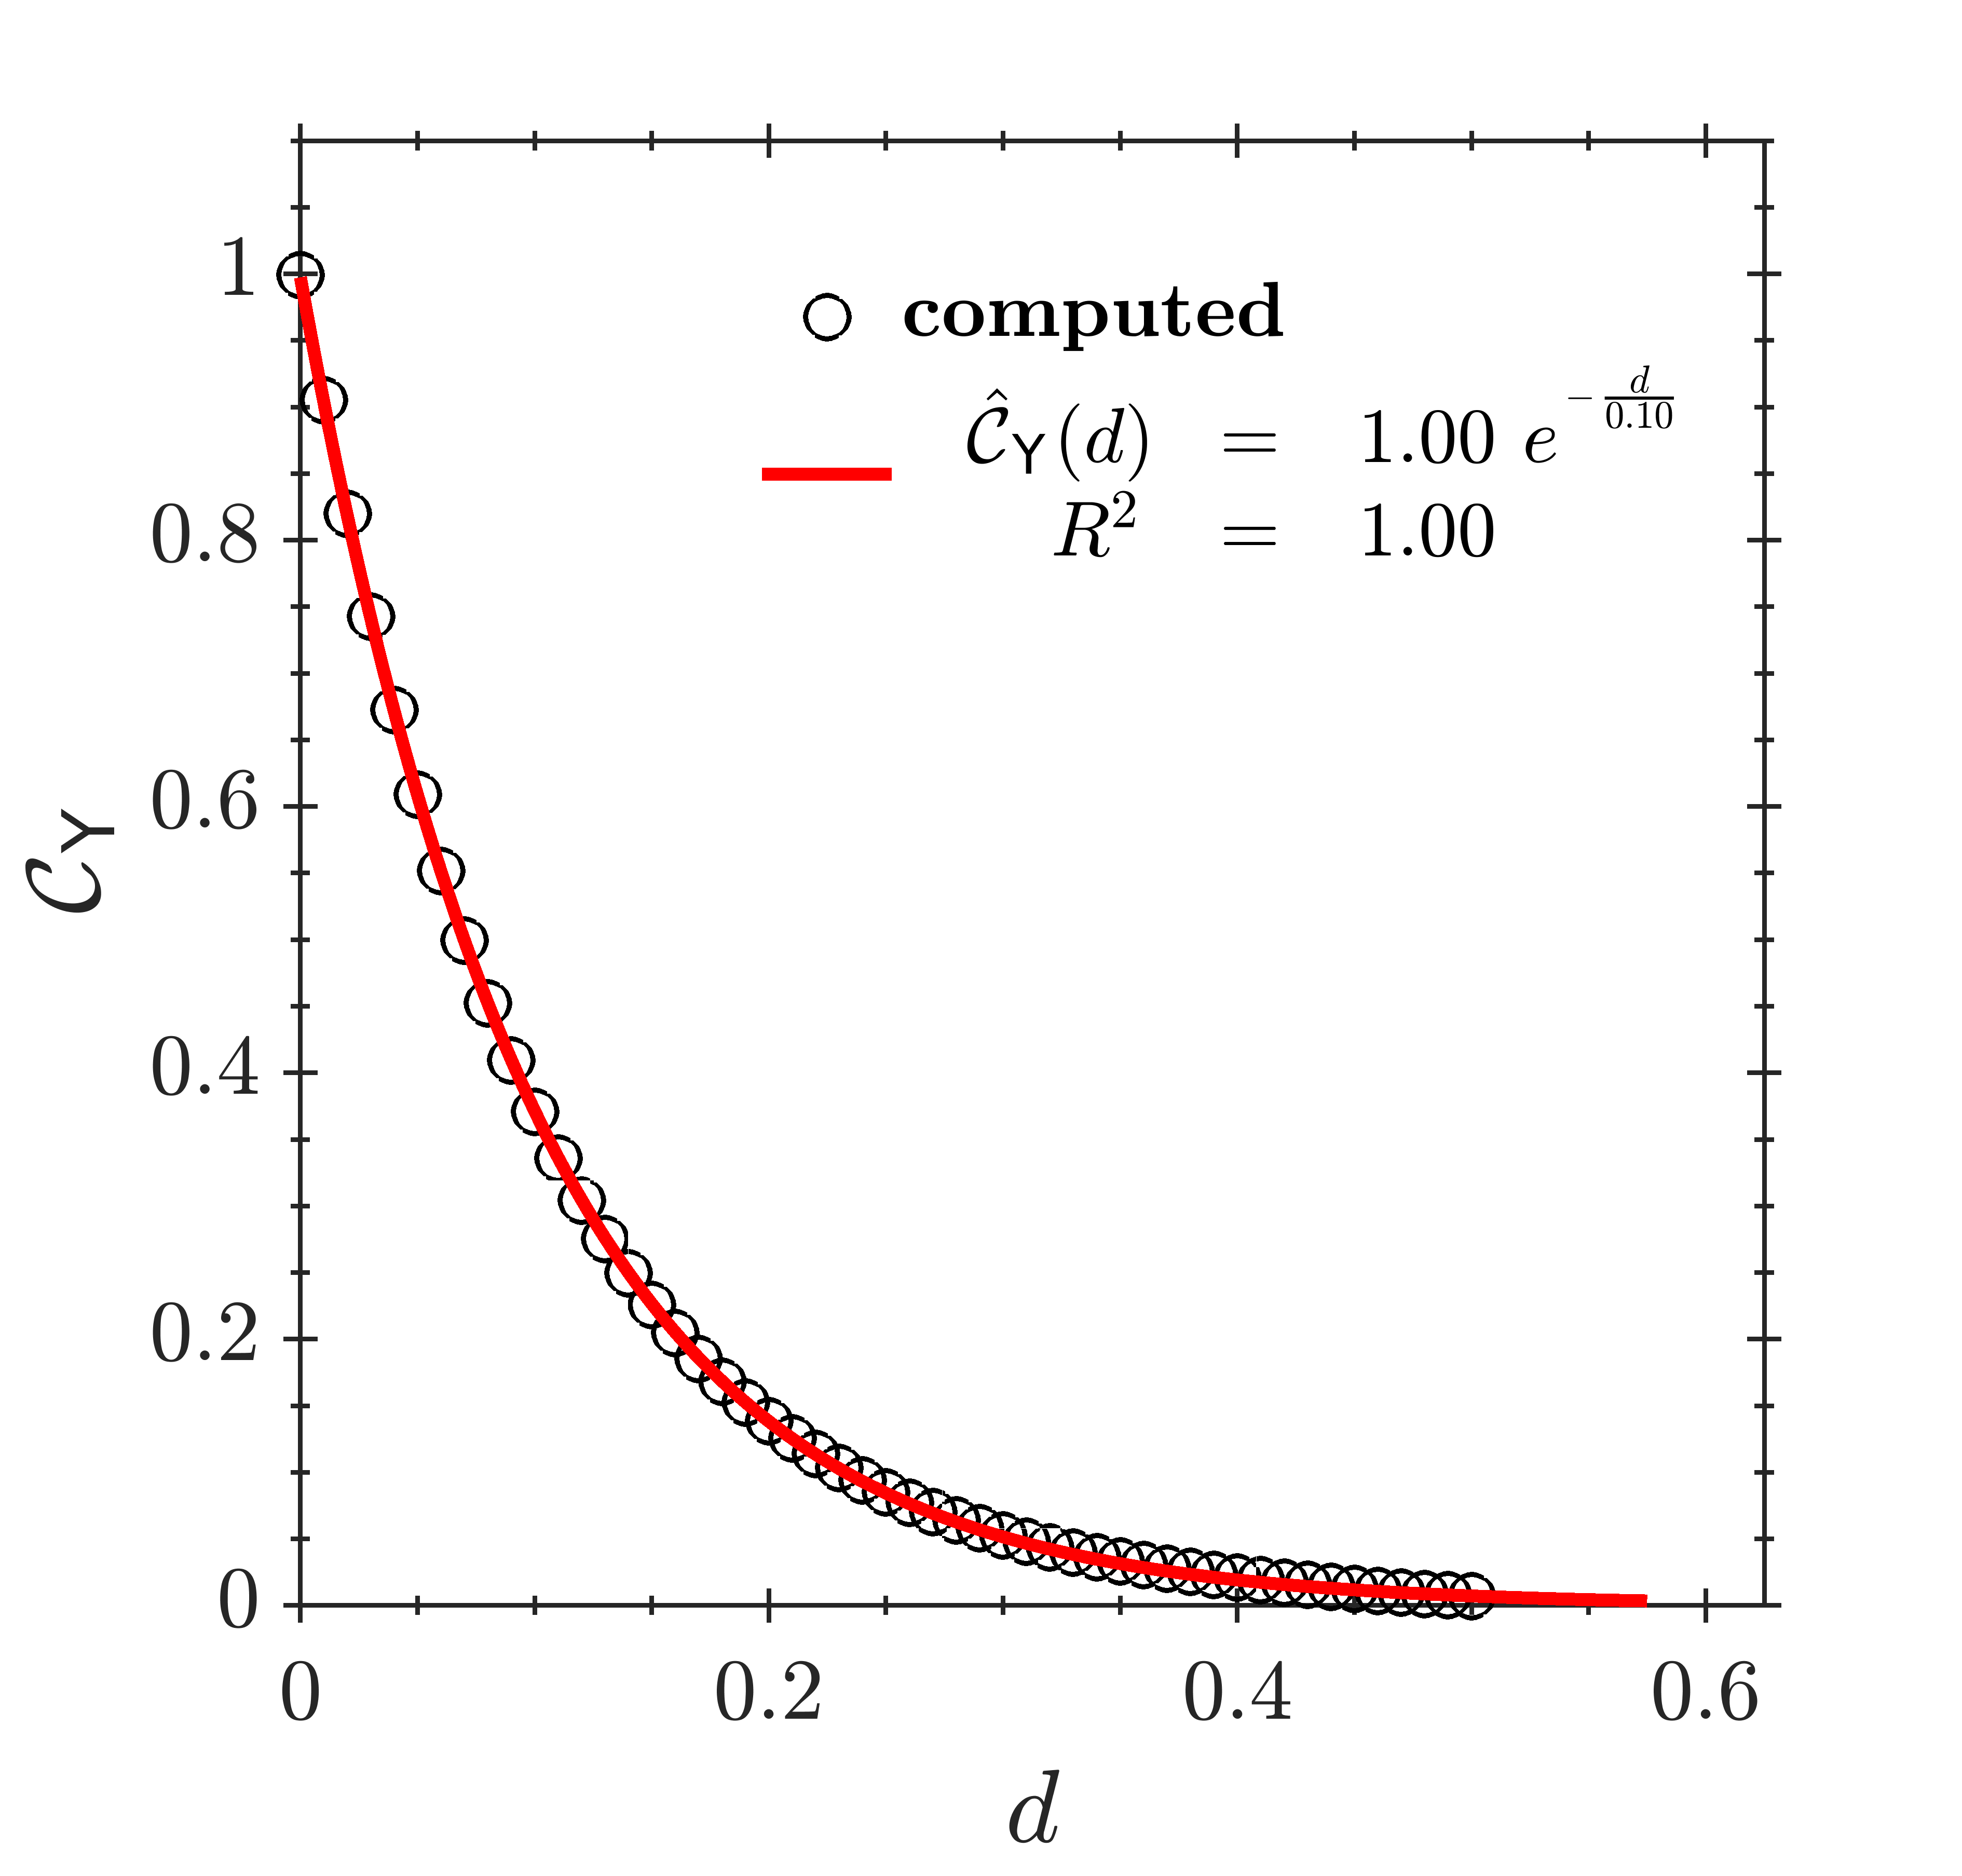
\includegraphics[scale=0.45]{./figuras/e_gsexp_1x1_100x100_0-1x0-1_5000_Yx.png}}
 \subfigure[$y$ direction]{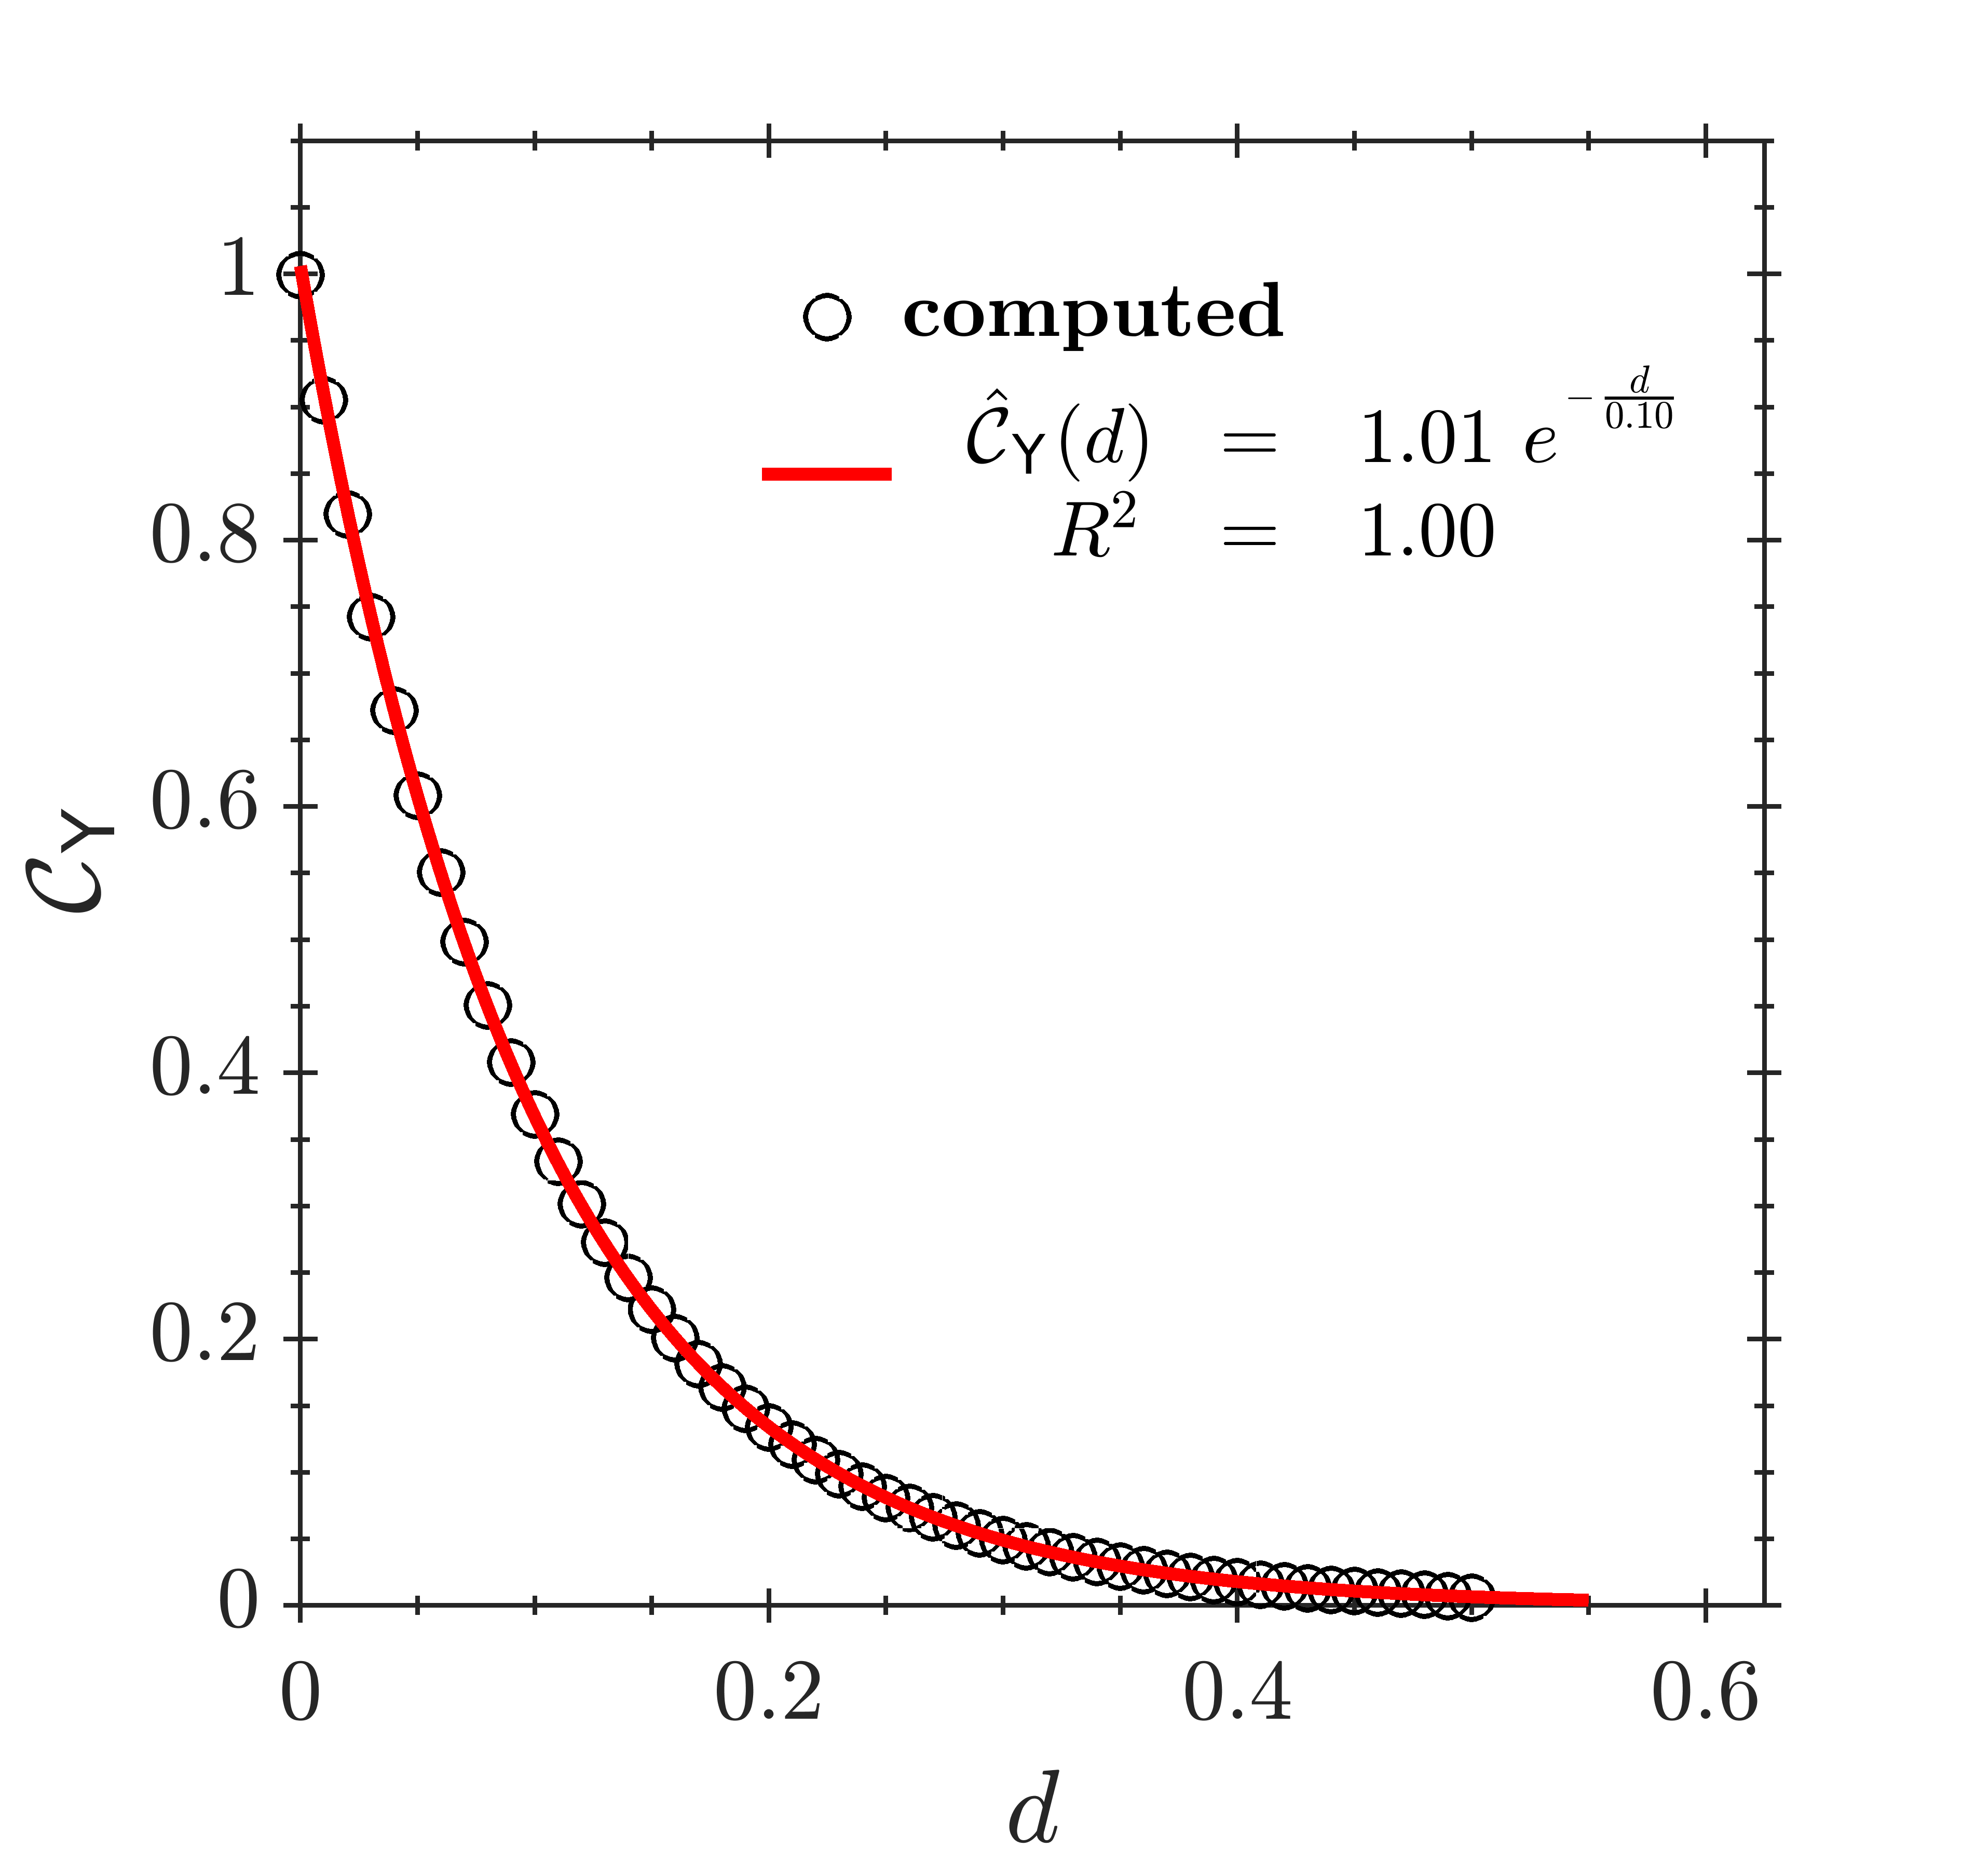
\includegraphics[scale=0.45]{./figuras/e_gsexp_1x1_100x100_0-1x0-1_5000_Yy.png}}
 \caption{Estimated covariance in a sample of $5,000$ fields generate by \kle\ with $30,000$ terms. Exponential case with $\clen = 0.1$.}
 \label{covar_expKL1}
\end{figure}

%%%%%%%%%%%%%%%%%%%%%%%%%%%%%%%%%%%%%%%%%%%%%%%%%%%%%%%%%%%%%%%%%%%%%%%%%%%%%%%%%%%%%%
\begin{figure}[H]
 \centering
 \subfigure[$x$ direction]{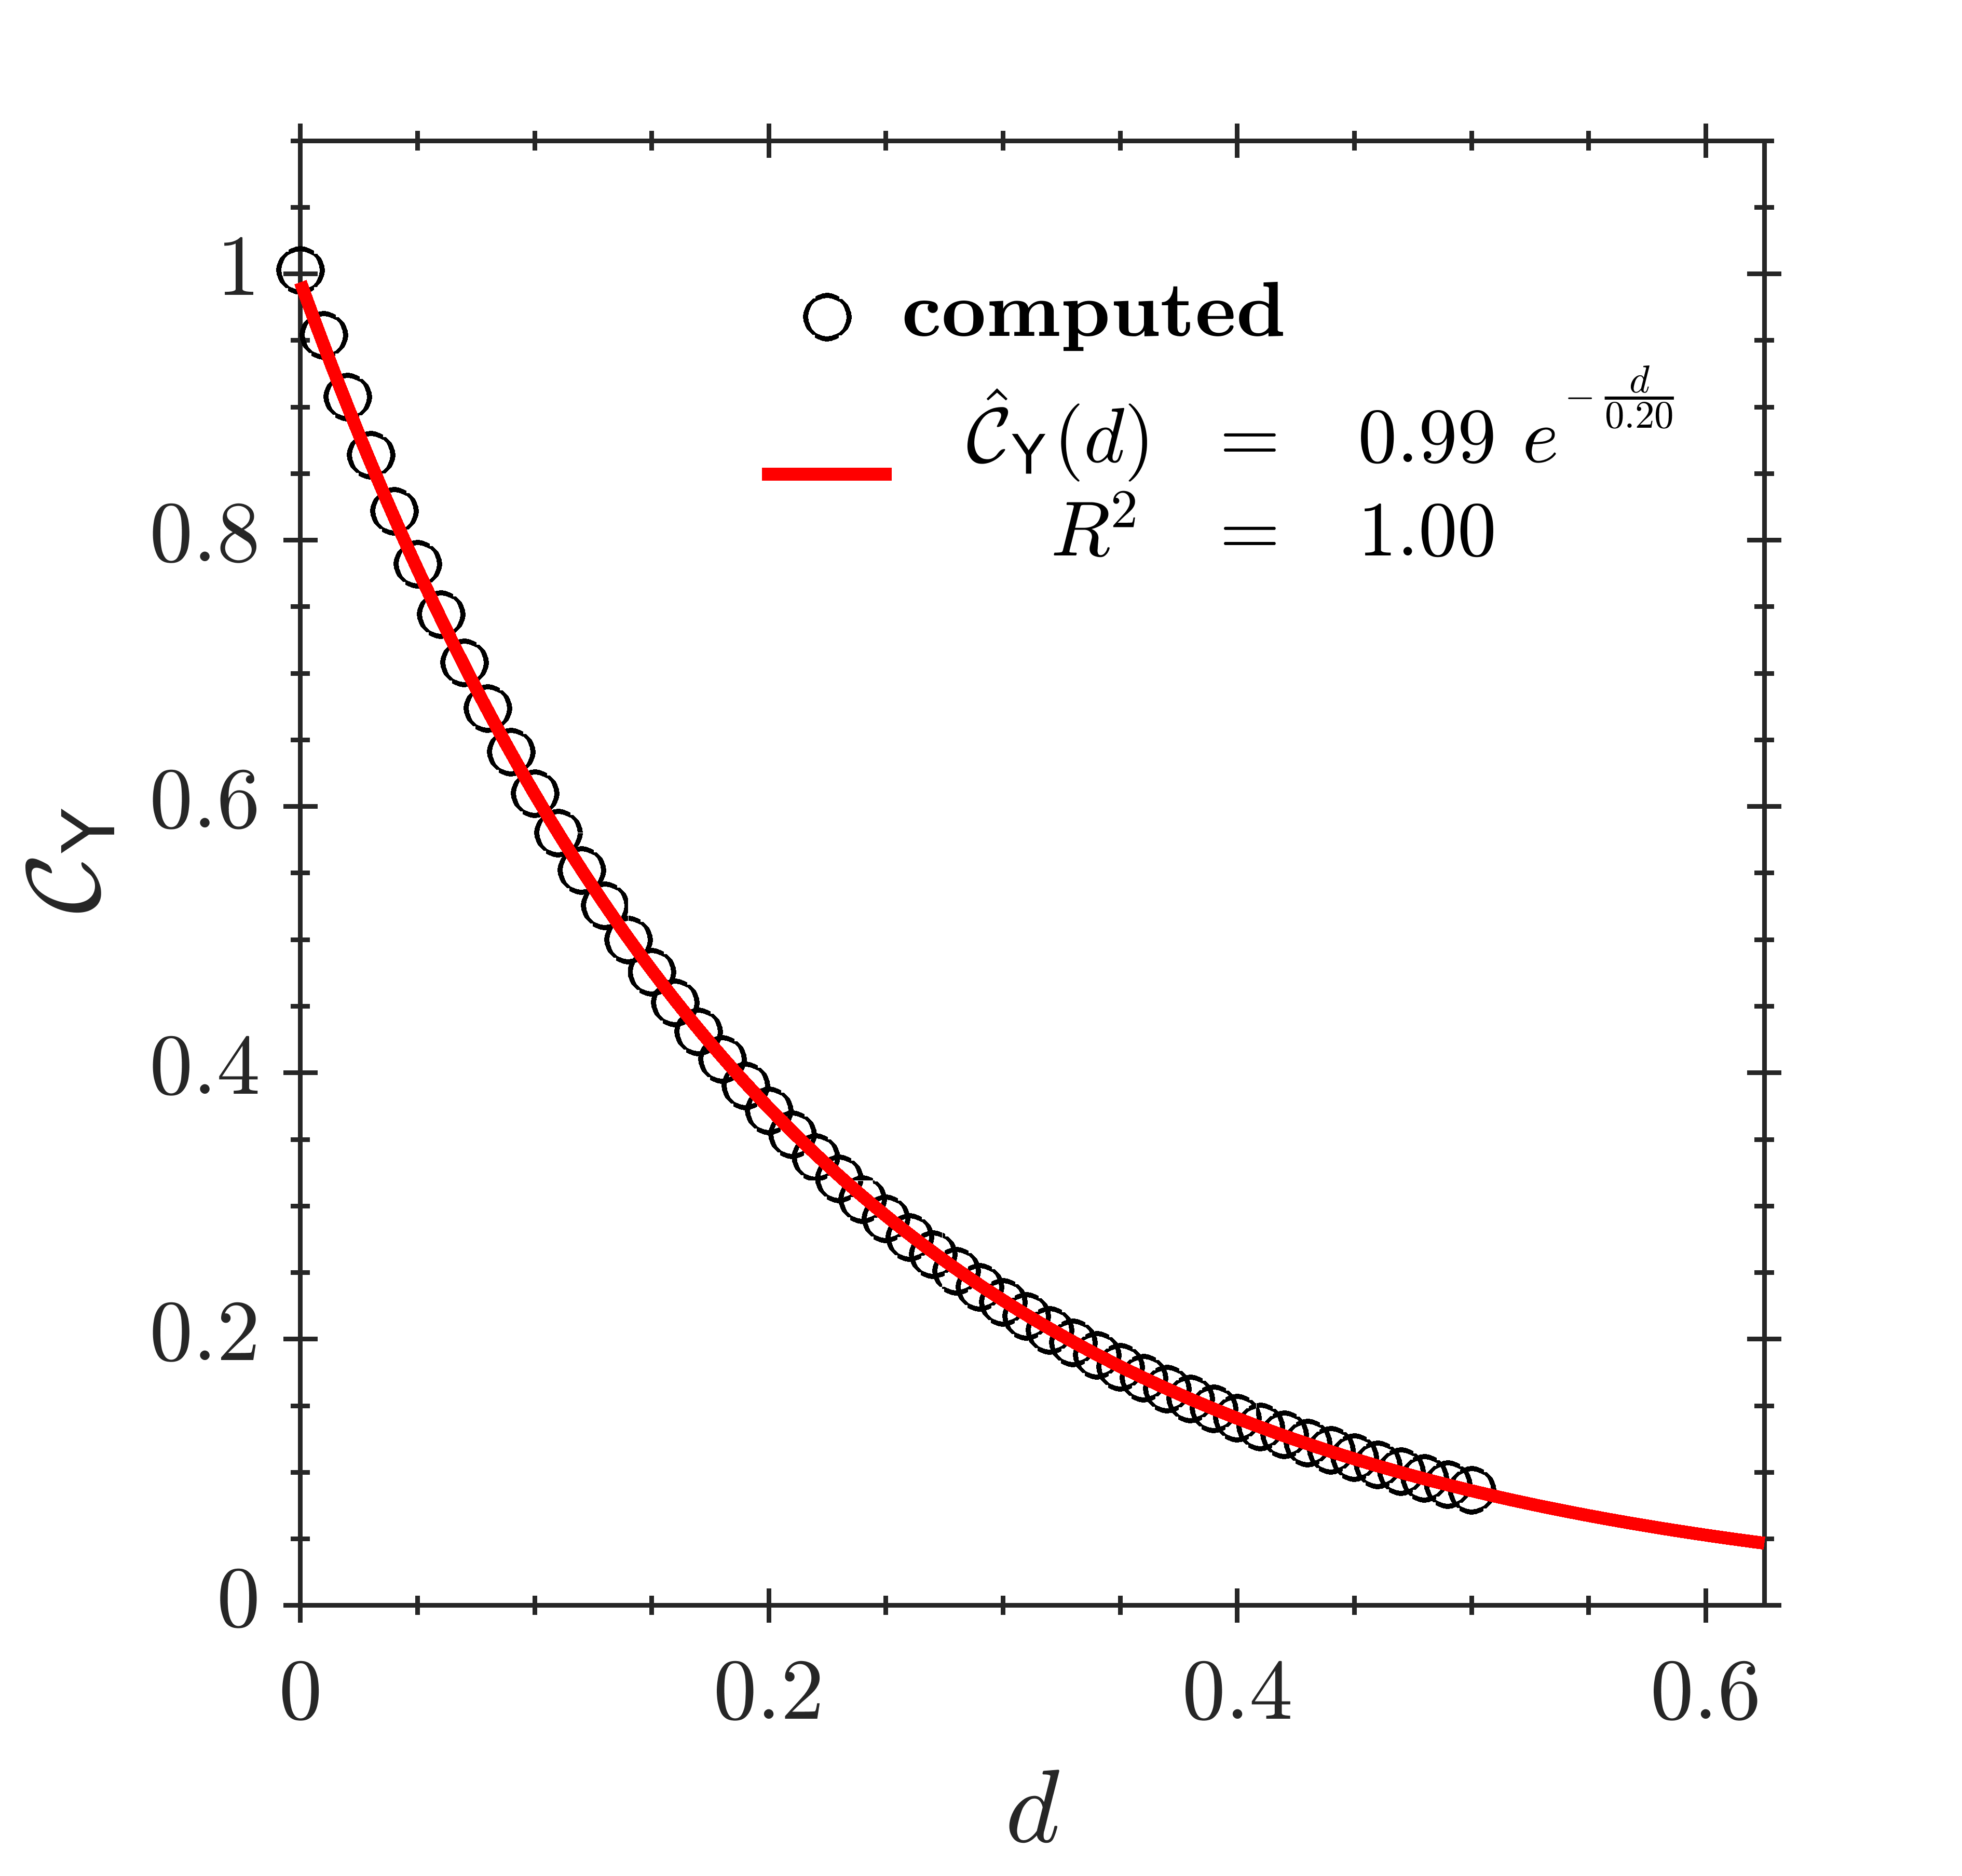
\includegraphics[scale=0.45]{./figuras/e_gsexp_1x1_100x100_0-2x0-2_5000_Yx.png}}
 \subfigure[$y$ direction]{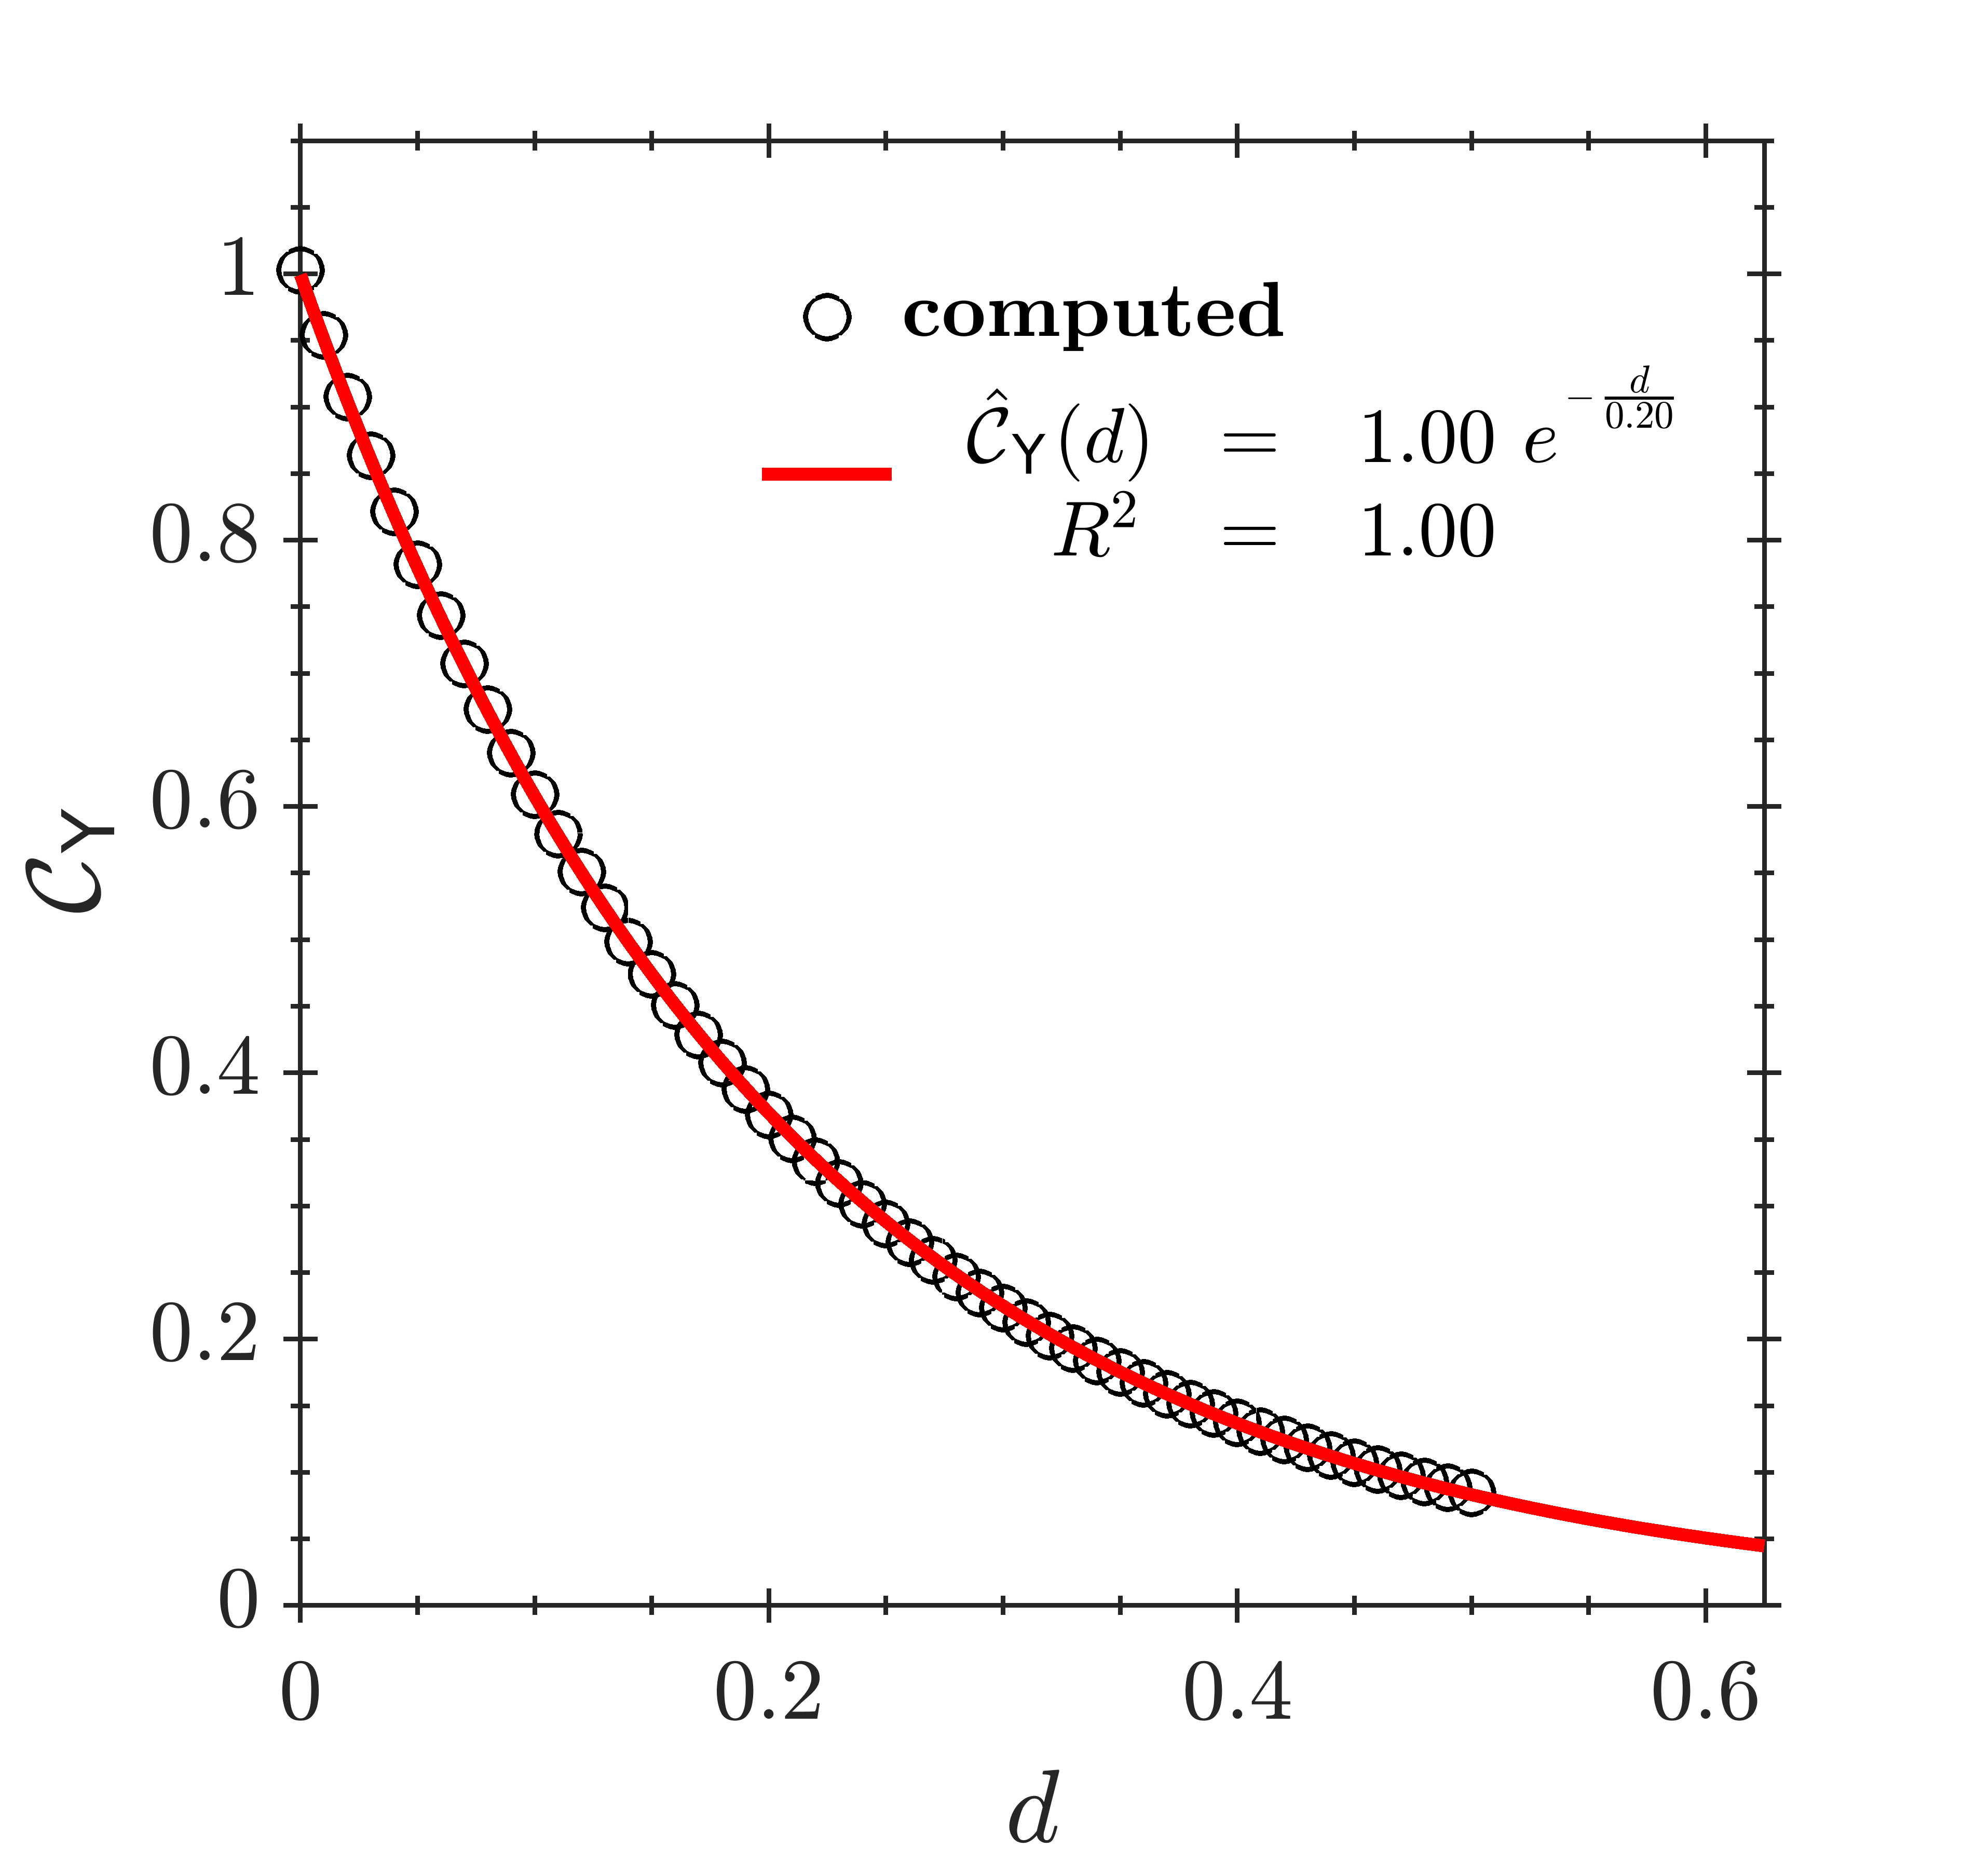
\includegraphics[scale=0.45]{./figuras/e_gsexp_1x1_100x100_0-2x0-2_5000_Yy.png}}
 \caption{Estimated covariance in a sample of $5,000$ fields generate by \kle\ with $30,000$ terms. Exponential case with $\clen = 0.2$.}
 \label{covar_expKL2}
\end{figure}

%%%%%%%%%%%%%%%%%%%%%%%%%%%%%%%%%%%%%%%%%%%%%%%%%%%%%%%%%%%%%%%%%%%%%%%%%%%%%%%%%%%%%%
%%%%%%%%%%%%%%%%%%%%%%%%%%%%%%%%%%%%%%%%%%%%%%%%%%%%%%%%%%%%%%%%%%%%%%%%%%%%%%%%%%%%%%
%%%%%%%%%%%%%%%%%%%%%%%%%%%%%%%%%%%%%%%%%%%%%%%%%%%%%%%%%%%%%%%%%%%%%%%%%%%%%%%%%%%%%%
%%%%%%%%%%%%%%%%%%%%%%%%%%%%%%%%%%%%%%%%%%%%%%%%%%%%%%%%%%%%%%%%%%%%%%%%%%%%%%%%%%%%%%
%%%%%%%%%%%%%%%%%%%%%%%%%%%%%%%%%%%%%%%%%%%%%%%%%%%%%%%%%%%%%%%%%%%%%%%%%%%%%%%%%%%%%%
%%%%%%%%%%%%%%%%%%%%%%%%%%%%%%%%%%%%%%%%%%%%%%%%%%%%%%%%%%%%%%%%%%%%%%%%%%%%%%%%%%%%%%
%%%%%%%%%%%%%%%%%%%%%%%%%%%%%%%%%%%%%%%%%%%%%%%%%%%%%%%%%%%%%%%%%%%%%%%%%%%%%%%%%%%%%%
%%%%%%%%%%%%%%%%%%%%%%%%%%%%%%%%%%%%%%%%%%%%%%%%%%%%%%%%%%%%%%%%%%%%%%%%%%%%%%%%%%%%%%
